\documentclass[a4paper,12pt,onecolumn,twoside]{article}
%%package
\usepackage[UTF8, heading = false, scheme = plain]{ctex} %中文支持
\usepackage{fancyhdr}
\usepackage{indentfirst} % 中文段落首行缩进
\usepackage{bm}          % 公式中的粗体字符(用命令\boldsymbol)
\usepackage{multicol}    % 正文双栏
\usepackage{indentfirst} % 中文首段缩进
\usepackage{graphicx} 
\usepackage{geometry}
\usepackage{caption}
\usepackage{subfigure} %子图片

\usepackage{tikz}%流程图
\usetikzlibrary{shapes,arrows,chains}%
\usepackage{xcolor}%
 
%%title

\title{使用GCode的激光振镜控制系统及其激光烧结3D打印应用}
\date{}
\begin{document}
\maketitle
\vspace{5in}
\begin{flushright}
\large{
	廖洽源\\
	高三级\\
	潮州市金山中学\\
	\today
}
\end{flushright}

\thispagestyle{empty}    %首頁頁碼空白
%%content
\tableofcontents
\newpage
\newgeometry{left=1in,right=1in,top=1in,bottom=1in} %更改边距

\twocolumn
%前言
\section{前言}
\subsection{激光打标}
激光打标是使用激光束在各种不同的物质表面打上永久的标记的过程的统称,电子元器件、集成电路(IC)、五金制品等都是用这种设备来为产品加上商标(二维矢量图).
\begin{figure}[ht]
\centering
\subfigure[常见激光打标机]{ 
\centering
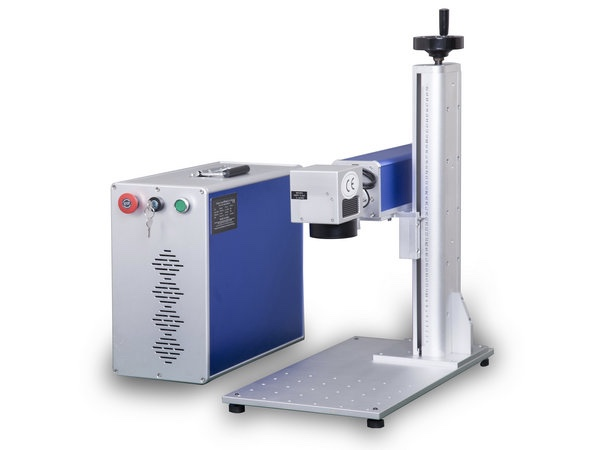
\includegraphics[width=0.9\linewidth]{MG0.jpg}
}
\subfigure[iPhone手机背面文字商标为激光打标制造]{
\centering     
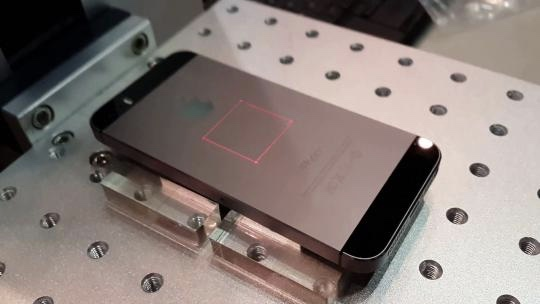
\includegraphics[width=0.9\linewidth]{MG1.jpg}
}
\caption{激光打标}
\end{figure}
\subsubsection{振镜电机}
振镜是一种优良的矢量扫描器件.它是一 种特殊的摆动电机,基本原理是通电线圈在磁场中 产生力矩 ,但与旋转电机不同,其转子上通过机械纽 簧或电子的方法加有复位力矩 ,大小与转子偏离平 衡位置的角度成正比 ,当线圈通以一定的电流而转子发生偏转到一定的角度时 ,电磁力矩与回复力矩大小相等 ,故不能象普通电机一样旋转 ,只能偏转,偏转角与电流成正比 ,与电流计的原理相同 ,故振镜又叫电流计扫描器(galvanometric scanner).
\begin{figure}[ht]
\centering
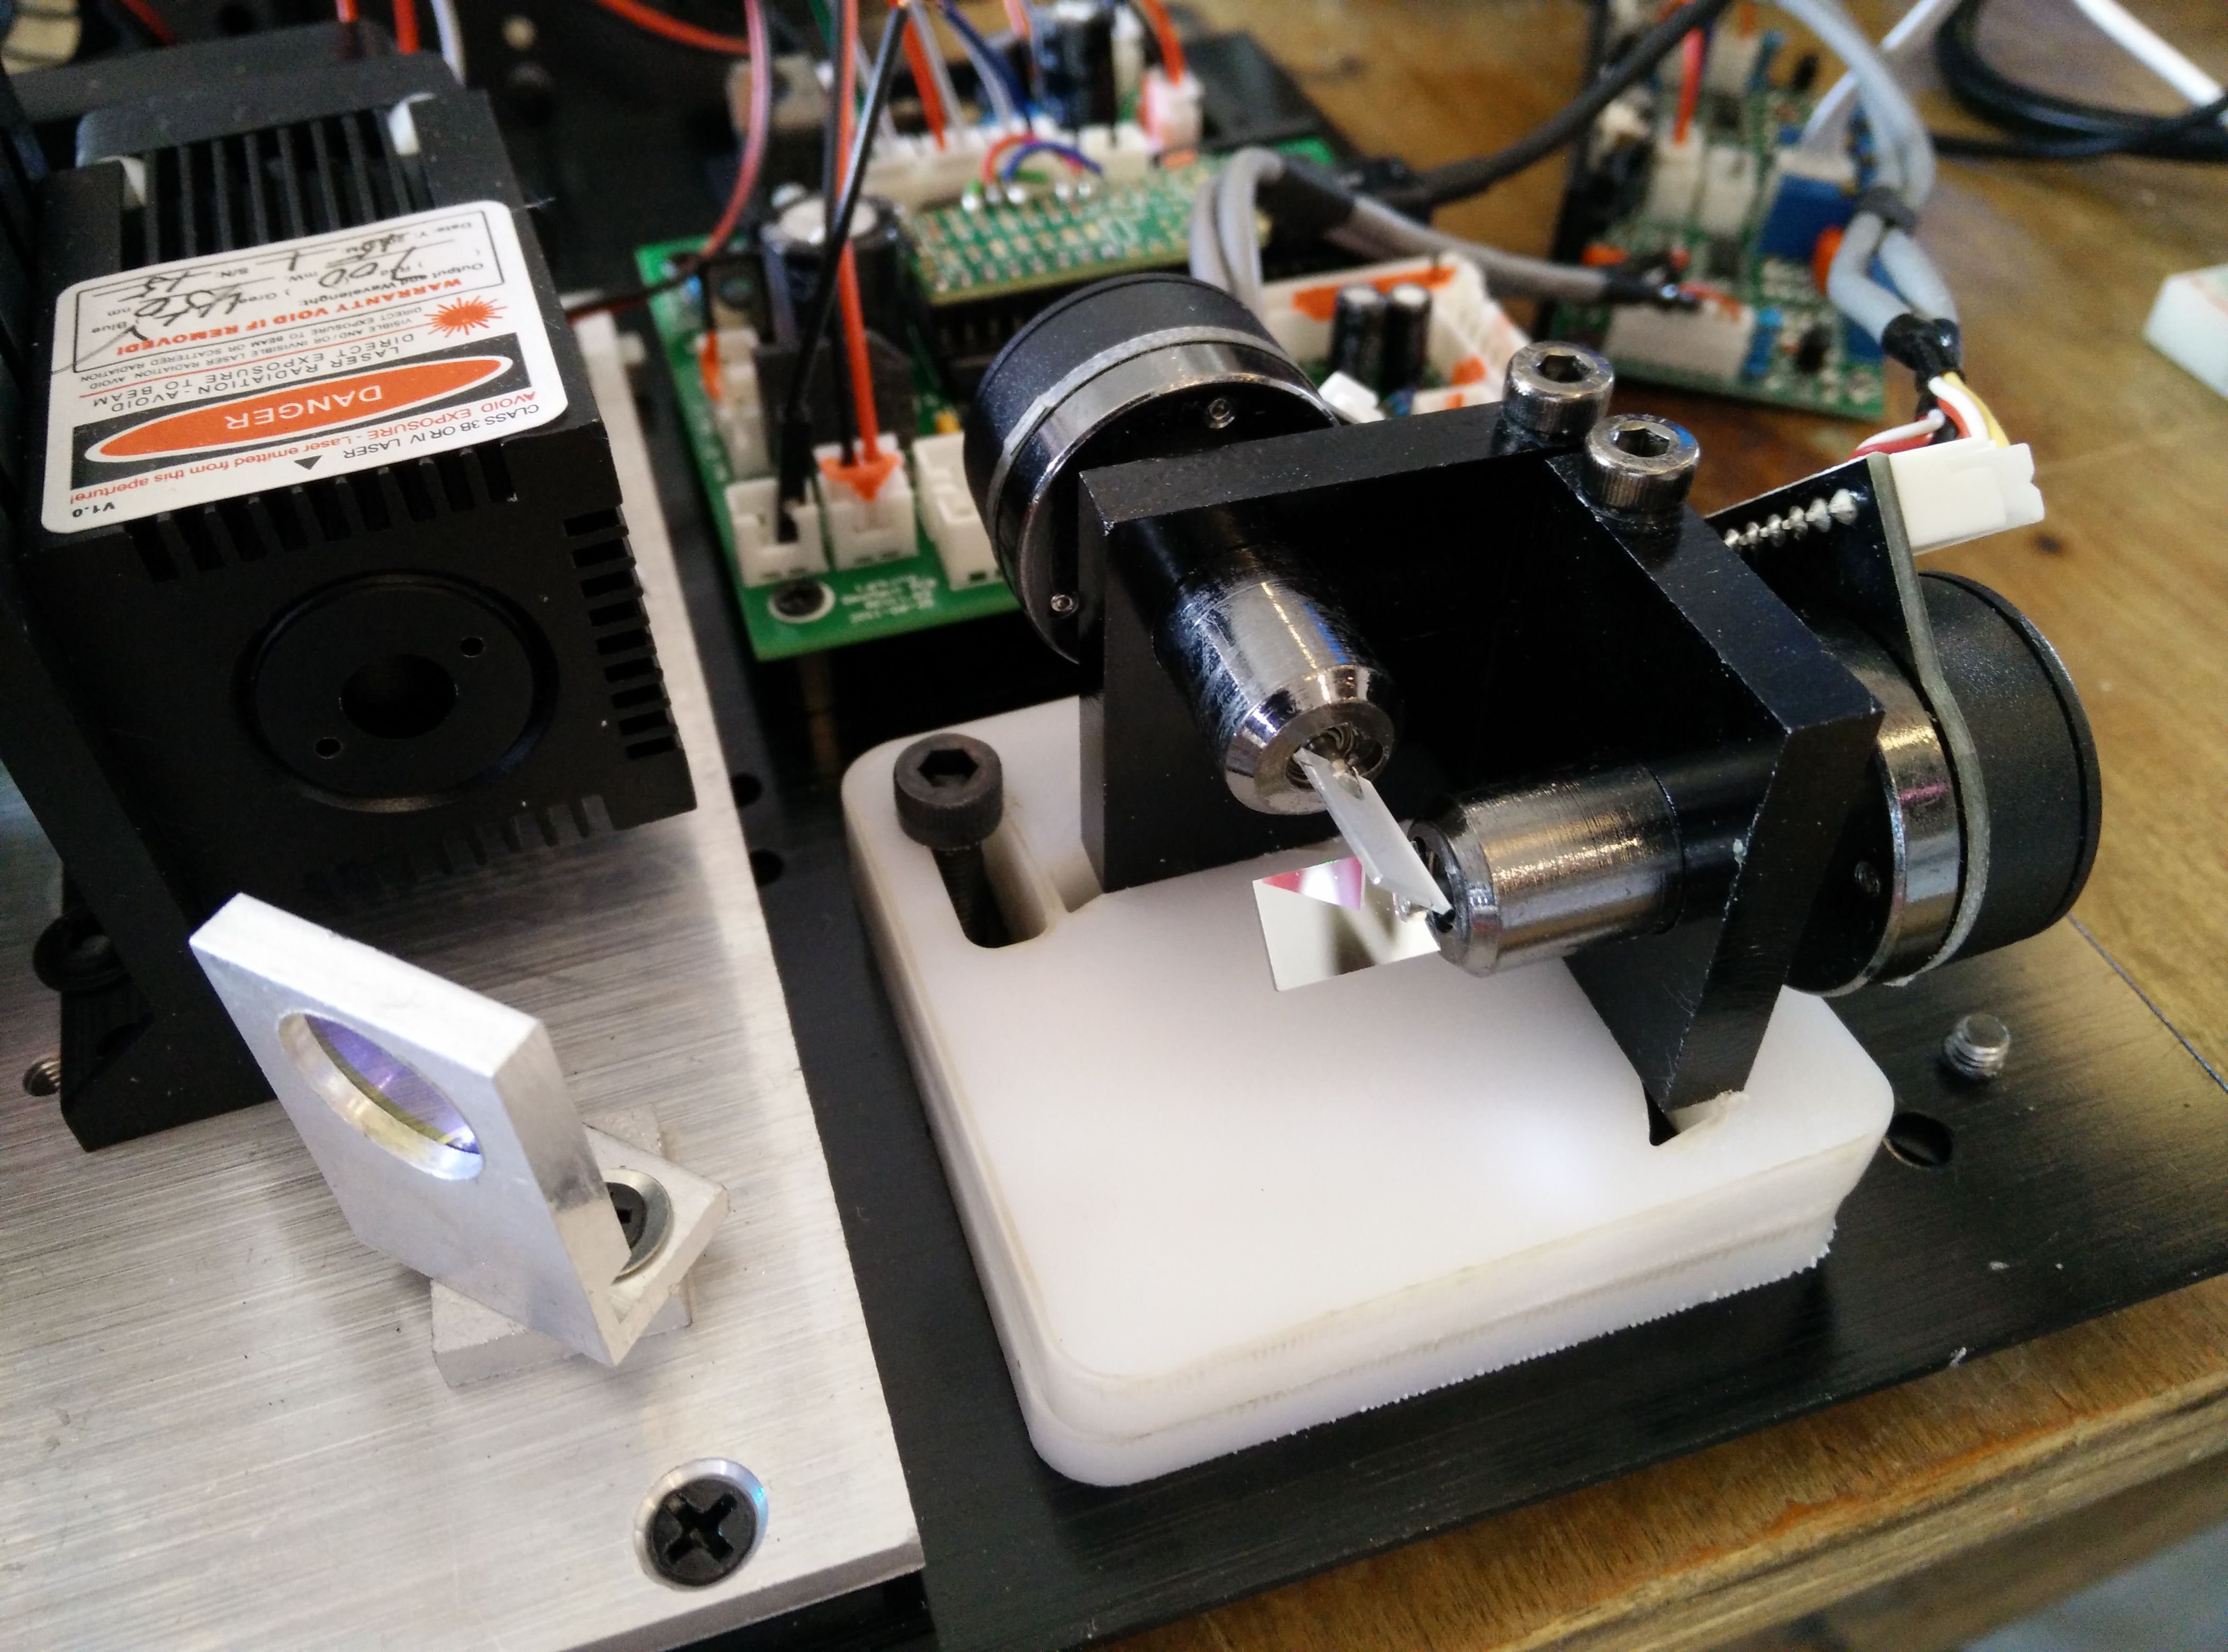
\includegraphics[width=\linewidth]{MG2.jpg}
\caption{两个振镜电机和激光器构成的XY二维扫描系统}
\end{figure}

\subsection{3D打印}
3D打印机又称三维打印机(3DP),是一种累积制造技术,即快速成形技术的一种机器,它是一种数字模型文件为基础,运用特殊蜡材、粉末状金属或塑料等可粘合材料,通过打印一层层的粘合材料来制造三维的物体.现阶段三维打印机被用来制造产品. 3D打印无需机械加工或模具,就能直接从计算机图形数据中生成任何形状的物体, 从而极大地缩短了产品的生产周期,提高了生产率,在工业(制造业、航天科技、医疗行业等)及民用(教育研究、生活用品等)领域有着许多应用.
\subsubsection{3D打印机原理概述}
3D打印的一般流程如下:
\paragraph{建模}
3D打印模型可以使用计算机辅助设计软件(SolidWorks、AutoCAD)或三维扫描仪生成.手动搜集制作3D图像所需的几何数据过程同雕塑等造型艺术类似.通过3D扫描,可以生成关于真实物体的形状、外表等的电子数据并进行分析.以3D扫描得到的数据为基础,就可以生成被扫描物体的三维电脑模型.
无论使用哪种3D建模软件,生成的3D模型(通常为.skp、.dae、.3ds或其它格式)都需要转换成.STL或.OBJ这类以三角形作为3D模型的基本单元的格式.
\paragraph{分层}
把模型放在XY平面上,Z轴对应的就是模型高度.把XY平面抬高一定高度再与模型的表面相交,就可以得到模型在这个高度上层切片.所谓的分层就是每隔一定高度就用一个XY平面去和模型相交作层切片,全部切完后就可以得到模型在每一个高度上的轮廓线.分层本质上就是一个把3D模型转化为一系列2D平面的过程,自此之后的所有操作就都是在2D图形的基础上进行.
将XY平面与构成模型的三角面进行相交,一个平面和一个三角形相交,就得到一条线段.将这些线段连起来 就能得到某Z轴高度的 XY轴外形轮廓.改变z轴高度便能得到不同层的外形轮廓.
\paragraph{路径及GCode生成}
得到外形轮廓后通过算法生成填充路径 后将路径转换成数控程序(铣床 车床 钻床等)通用的G代码.
\begin{figure}[ht]
\centering
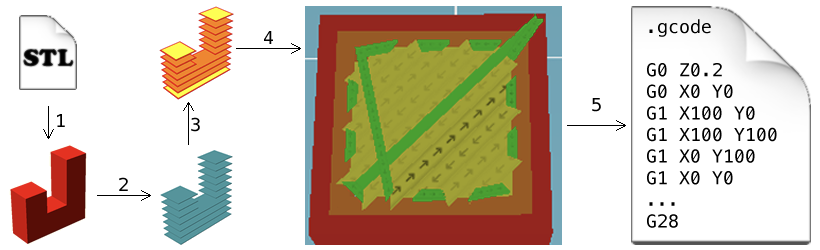
\includegraphics[width=0.9\linewidth]{stlToGcode.png}
\caption{电脑上的处理过程}
\end{figure}
\subsubsection{常见3D打印机成型原理细分}
在20世纪70年代后期,出现了许多不同的3D打印方法,主要有三种熔融沉积成型(FDM)、
立体光刻技术(SLA)、选择性激光烧结术(SLS)
\paragraph{熔融沉积成型(Fused deposition modeling, FDM)}
是一种将各种热熔性的丝状材料(ABS和PLA等)加热熔化成形的方法.又可被称为FFM 熔丝成型 (Fused Filament Modeling) 或FFF 熔丝制造 (Fused Filament Fabrication),其后两个不同名词主要只是为了避开前者FDM专利问题,然而核心技术原理与应用其实均是相同的.
材料被加热到半液体状态后,在GCode的控制下,FDM装置的喷嘴就会沿着模型图的表面移动,将热塑性材料挤压出来,在该层中凝固形成轮廓.FDM 装置会使用两种材料来执行打印的工作,分别是用于构成成品的建模材料和用作支架的支撑材料,透过喷嘴垂直升降,材料层层堆积凝固后,就能由下而上形成一个3D打印模型的实体.打印完成实体.
\begin{figure}[ht]
\centering
\subfigure[1为喷头 2为打印半完成的零件 3为底板]{
\centering     
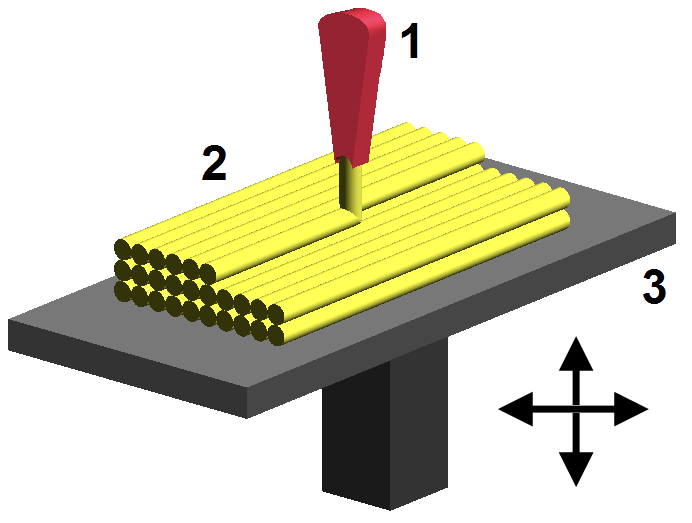
\includegraphics[width=0.9\linewidth]{FDM0.png}
}
\subfigure[另一个视角]{ 
\centering
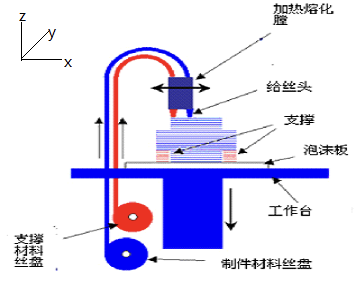
\includegraphics[width=0.9\linewidth]{FDM1.png}
}
\caption{FDM3D打印原理}
\end{figure}
\subparagraph{优点}
在3D打印技术中,FDM的机械结构最简单,设计也最容易,制造成本、维护成本和材料成本也最低,因此桌面级3D打印机中大部分使用的是这种技术.
\subparagraph{缺点}
难以精确控制出料形态与成型效果,同时温度对于FDM成型效果影响非常大,而桌面级FDM 3D打印机通常都缺乏恒温设备,因此基于FDM的桌面级3D打印机的成品精度通常为0.3mm-0.2mm成品效果依然不够稳定,在打印悬空结构时还必须从一开始便构建“支撑”,导致精度进一步降低.此外,所以在对精度要求较高的快速成型领域较少采用FDM.
\begin{figure}[ht]
\centering
\subfigure[不打印支撑时对模型的要求]{
\centering     
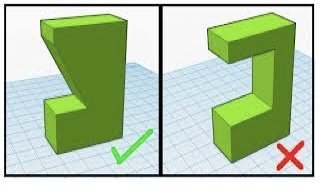
\includegraphics[width=0.9\linewidth]{FDM2.jpg}
}
\subfigure[支撑去除前后对比(白色为支撑)]{ 
\centering
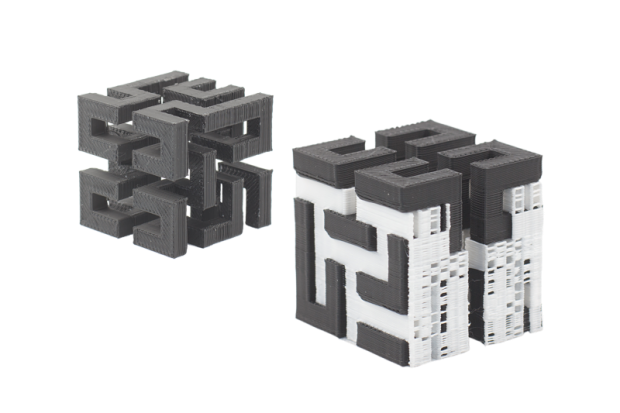
\includegraphics[width=0.9\linewidth]{FDM3.png}
}
\caption{FDM对于零件的要求}
\end{figure}
\\
\paragraph{选择性激光烧结(Selective Laser Sintering,SLS)}
选择性激光烧结使用激光将粉末材料层熔化和固化成成品,当激光打到粉末上,粉末会融化并且和附近粉末粘在一起,当激光在粉末层上匀速扫过一条直线时,粉末便会固化成一条细丝,激光不断扫描出面时,粉末便可以被固化成面,在形成的面上面再铺一层粉末,激光继续扫描,不断重复这个过程,就能得到一个3D零件.
\begin{figure}[ht]
\centering     
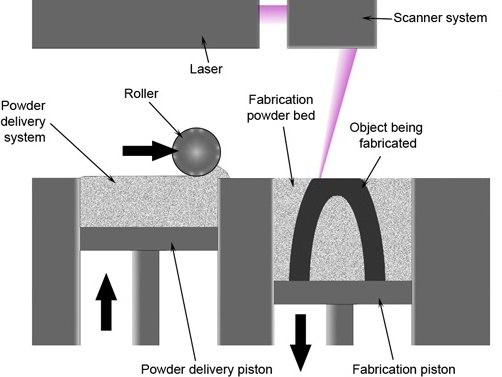
\includegraphics[width=0.9\linewidth]{SLS0.jpg}
\caption{SLS3D打印原理}
\end{figure}
\subparagraph{优点}
SLS主要用于工业3D打印应用,激光烧结技术可以使用非常多的粉末材料,并制成相应材质的成品SLS广泛用于生产功能原型和零件以及一些最终产品. 激光烧结的最大优点是几乎完全的设计自由度; 过量的未熔化粉末在其生产时用作结构的支撑,这允许制造复杂的结构,而不需要像FDM SLA DLP等构建额外的支撑.
\subparagraph{缺点}
技术十分复杂,需要较大功率激光,桌面级的SLS3D打印机只少量存在于高校或团队. 
\subsection{同类项目}
\subsubsection{现存桌面级SLS3D打印机}
现存的桌面级SLS3D打印机都是在FDM3D打印机(或者激光切割机)基础上改装而成,XY轴都是使用步进电机+同步带或丝杠的方式拖着激光器进行直线运动,这种机构的最大运动速度只能到达200mm/s左右.
\paragraph{OpenSLS项目}
由美国莱斯大学约旦米勒生理系统和先进材料实验室开发.这个项目的研究的主要方向为粉末烧结材料,是用一台CO2切割机改装而成.
\begin{figure}[ht]
\centering     
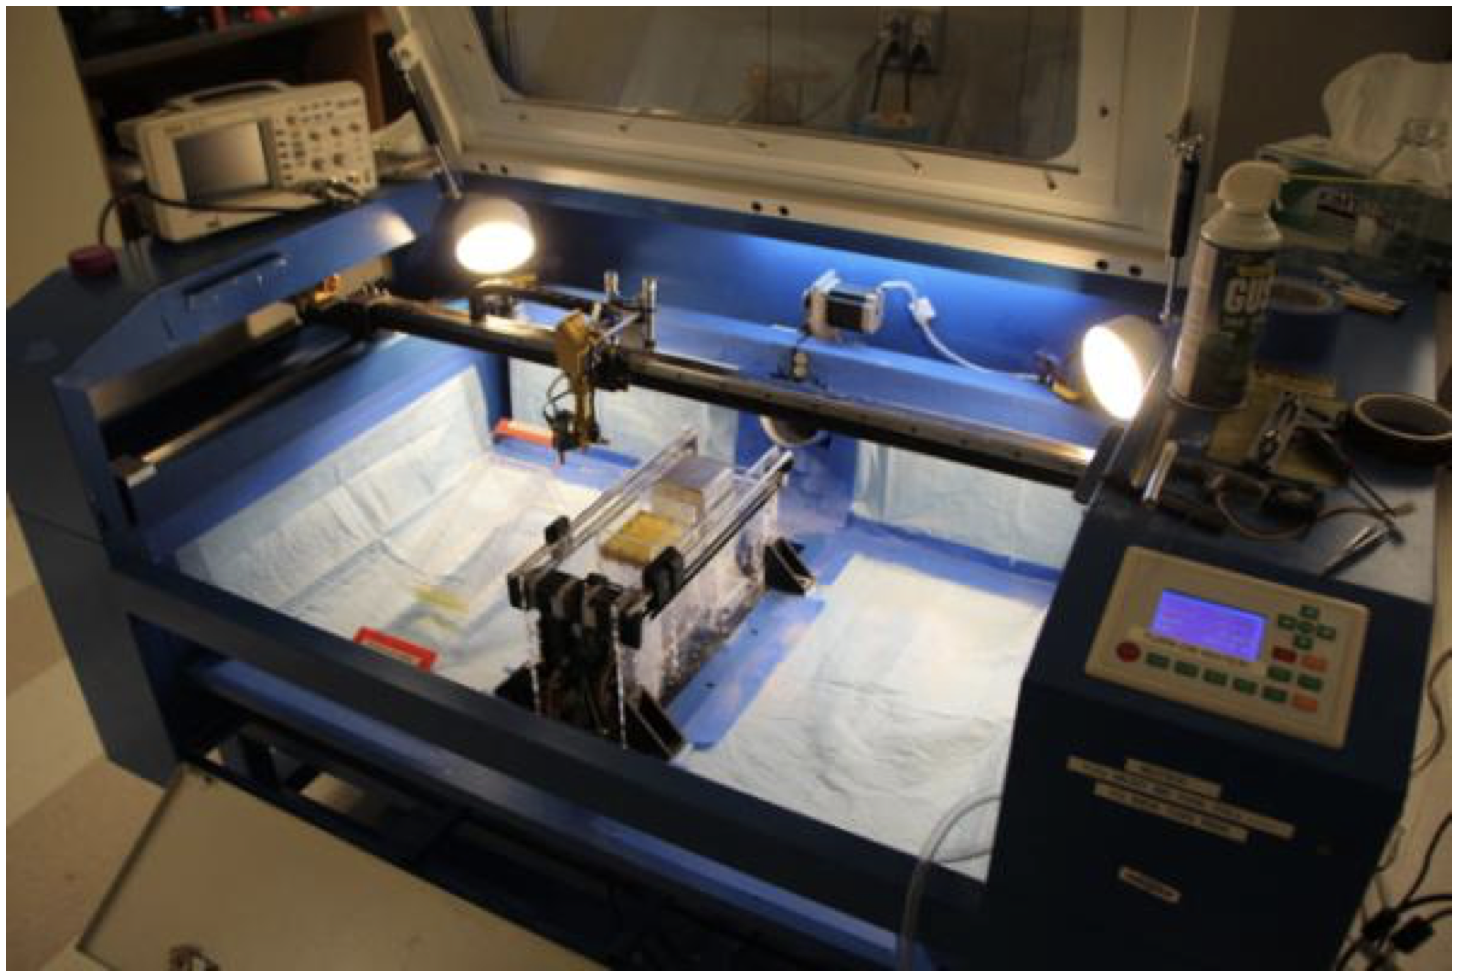
\includegraphics[width=0.8\linewidth]{OpenSLS0.png}
\centering
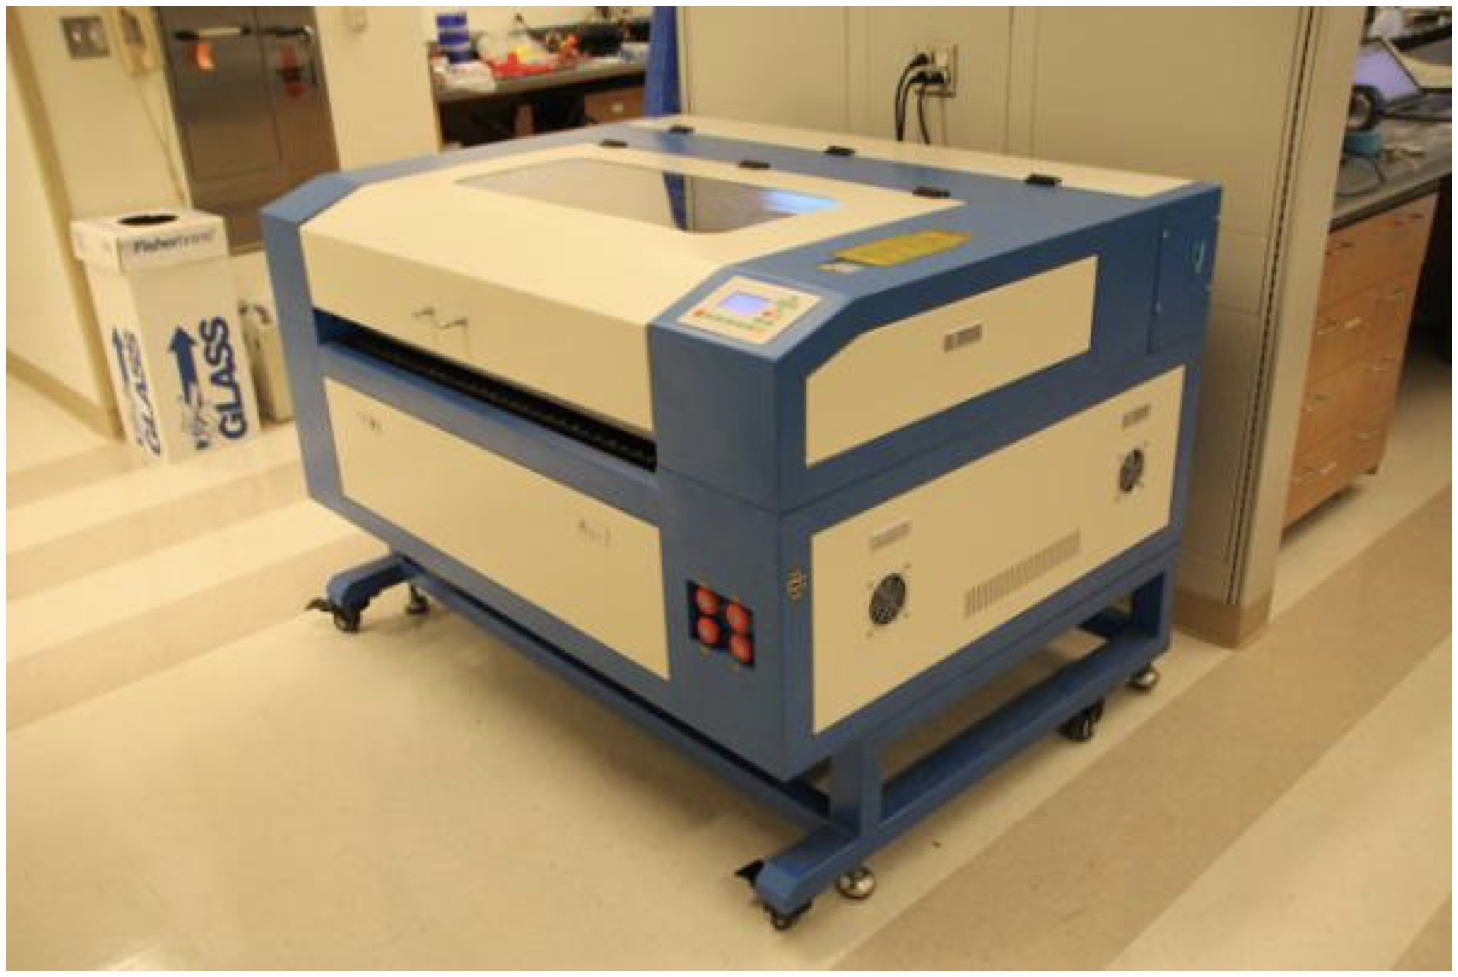
\includegraphics[width=0.8\linewidth]{OpenSLS1.png}
\caption{OpenSLS}
\end{figure}
\newpage

\begin{figure}[ht]
\centering
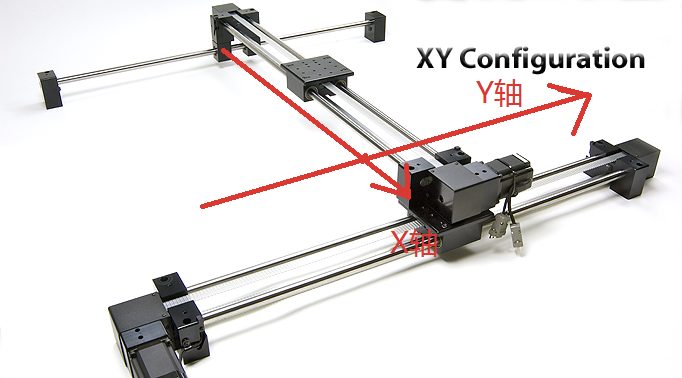
\includegraphics[width=0.9\linewidth]{OpenSLS2.png}
\caption{步进电机直线模组}
\end{figure}
\subsection{本项目简介}
\paragraph{选题动机}
步进电机直线模组的最大运动速度只能到达200mm/s左右,换言之,激光光斑的移动速度最大只有200mm/s,而激光打标机的振镜电机进行扫描速度能达到1000mms-5000mm/s,是步进电机直线模组的几十倍,为什么不把激光打标机的执行器(两个振镜组成的振镜组)用在SLS3D打印机上面???激光打标机使用的是二维矢量图不能适用于于3D打印,所以开发一个使用Gcode控制的振镜扫描系统是最佳的选择.
\paragraph{目标}
开发一个运行在Arduino Due单片机上的控制程序及配套硬件,可以用数控设备通用的G代码控制振镜,使得振镜兼容常规切片软件,可以用于SLS3D打印,并在此基础上研制使用振镜电机作为XY轴的桌面级SLS3D打印机.
\paragraph{实现方法}
在PC上使用切片软件将3D模型转换成GCode,每行GCode包含了运动轨迹的信息,将GCode通过串口发送到Arduino控制器上,Arduino控制器对GCode进行解释,判断是否需要进行烧结和移动粉缸和改变预热温度的操作及操作数值,对其进行进一步规划后执行,后对PC进行应答而获取下一行GCode,不断执行直至打印完成.
\newpage
%控制理论
\section{控制理论及实现}
本章介绍本项目中振镜电机的控制及补偿算法和步进电机加速度算法.
\subsection{振镜扫描控制}
\subsubsection{单轴振镜电机直线扫描控制}
\paragraph{条件}
设一垂直于振镜旋转轴的直线及原点,反射镜面与直线夹角$\frac{\pi}{4}$,运动目标点坐标x,振镜中心与原点距离d且在原点正上方,反射镜偏角$\alpha$
\begin{figure}[ht]
\centering     
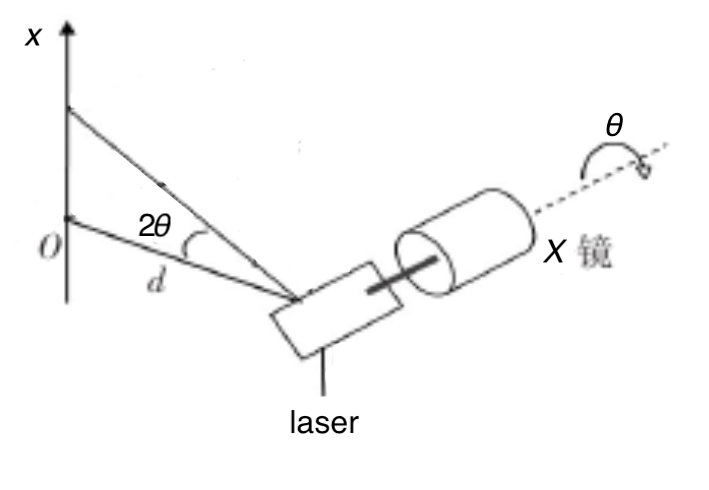
\includegraphics[width=\linewidth]{MG3.png}
\caption{单轴振镜电机示意图}
\end{figure}
\subparagraph{正运动学:}
\begin{equation}
x=d\tan2\alpha 
\end{equation}
\subparagraph{逆运动学:}
\begin{equation}
\alpha =\frac{1}{2}\arctan\frac{x}{d}
\end{equation}
\paragraph{控制要求}
\subparagraph{输入:}
运动目标点坐标$x$
\subparagraph{输出:}
反射镜偏角$\theta$
\paragraph{控制函数}即逆运动学
\begin{equation}
f(x)=\theta =\frac{1}{2} \arctan\frac{x}{d}
\end{equation}
\clearpage
\subsubsection{双轴振镜电机组平面扫描控制}

\paragraph{条件}
如果简单地使用单轴振镜电机的控制方法

\begin{figure}[ht]
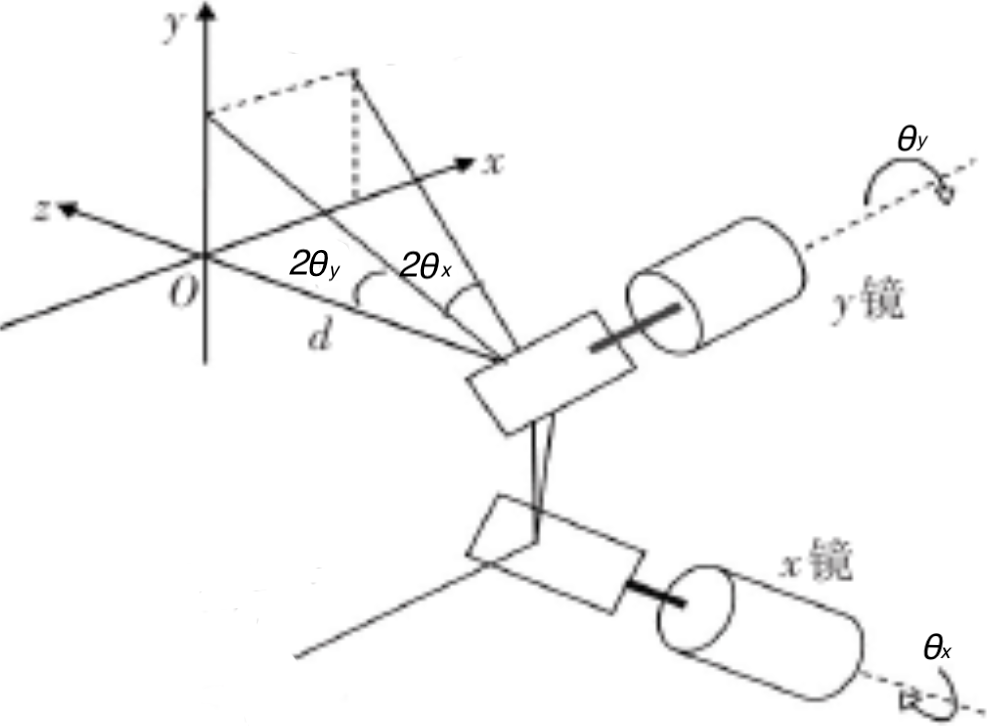
\includegraphics[width=1\linewidth]{MG4.png}
\caption{双轴振镜电机组示意图}
\end{figure}

\subparagraph{正运动学:}
\begin{equation}
\left\{
\begin{array}{c}
x=d\tan2\theta_x \\
y=d\tan2\theta_y\\ 
\end{array}
\right.
\end{equation}
\subparagraph{逆运动学:}
\begin{equation}
\left\{
\begin{array}{l}
2\theta_x = \arctan\frac{x}{d}  \\
2\theta_y = \arctan\frac{y}{d} \\
\end{array}
\right.
\end{equation}
 \paragraph{控制要求}
\subparagraph{输入:}
运动目标点坐标$(x,y)$
\subparagraph{输出:}
x轴振镜反射镜偏角$\theta_x$ , y轴振镜反射镜偏角$\theta_y$
\paragraph{控制函数}
\begin{equation}
f(x,y)=
\left\{
\begin{array}{l}
\theta_x = \frac{1}{2}\arctan\frac{x}{d}  \\
\theta_y = \frac{1}{2}\arctan\frac{y}{d} \\
\end{array}
\right.
\end{equation}
但是如果使用这种控制方式,y轴将会产生枕型失真.
\begin{figure}[ht]
\centering
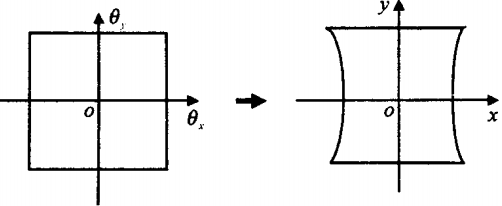
\includegraphics[width=\linewidth]{MG5.png}
\caption{扫描正方形图形的枕型失真}
\end{figure}
\newpage
使用上述控制方式控制双轴的振镜组,没有考虑到两个振镜的距离
\paragraph{条件}
设$x$振镜和$y$振镜反射镜中轴之间的距离为$e$,$y$振镜的轴线到扫描平面坐标原点的距离为d,当$x$,$y$轴的光学偏转角分别为$\theta_x$和$\theta_y$时,扫描平面上相应激光斑坐标为$(x,y)$,当$\theta_x=\theta_y=0$时,
\begin{figure}[ht]
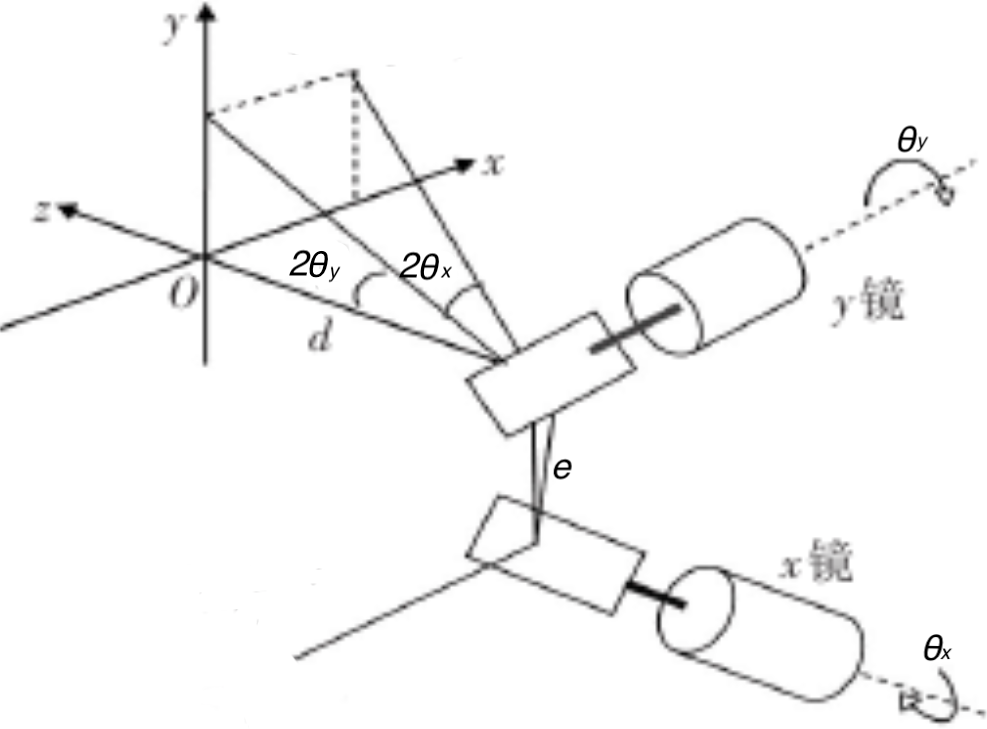
\includegraphics[width=\linewidth]{MG6.png}
\caption{双轴振镜电机组示意图}
\end{figure}
\subparagraph{正运动学:}
\begin{equation}
\left\{
\begin{array}{l}
x=(e+\sqrt{d^2+y^2})\tan 2\theta_x \\
y=d\tan 2\theta_y \\
\end{array}
\right.
\end{equation}
\subparagraph{逆运动学:}
\begin{equation}
\left\{
\begin{array}{l}
2\theta_x = \arctan \frac{x}{e+\sqrt{d^2+y^2}}  \\
2\theta_y = \arctan \frac{y}{d} \\
\end{array}
\right.
\end{equation}
可见,双轴振镜组的运动学模型是复杂的非线性模型.
\newpage
\subsubsection{双轴振镜电机失真分析}
\paragraph{失真产生}
使用单轴扫描方式控制双轴振镜组扫描垂直于x轴的直线时,$\theta_x$不变,设常数$c=2\tan\theta_x$
由$(7)$可得
\begin{equation}
\frac{(x-ce)^2}{c^2 d^2}-\frac{y^2}{d^2}=1
\end{equation}
显然$(9)$描述的曲线为双曲线\\
定义$\varepsilon$为误差 $x_0$为预期位置$x$为实际位置,可见当$e$和$x_0$越大时,x轴偏移$\varepsilon$将越大
\begin{equation}
\varepsilon=x-x_0=(e+\sqrt{d^2+e^2})\tan2\theta_x
\end{equation}
\paragraph{验证}
使用Matlab软件仿真扫描,当$e=5mm$,$d=200mm$扫描长宽为$50mm$的正方形图案\\
\begin{figure}[h]
\centering
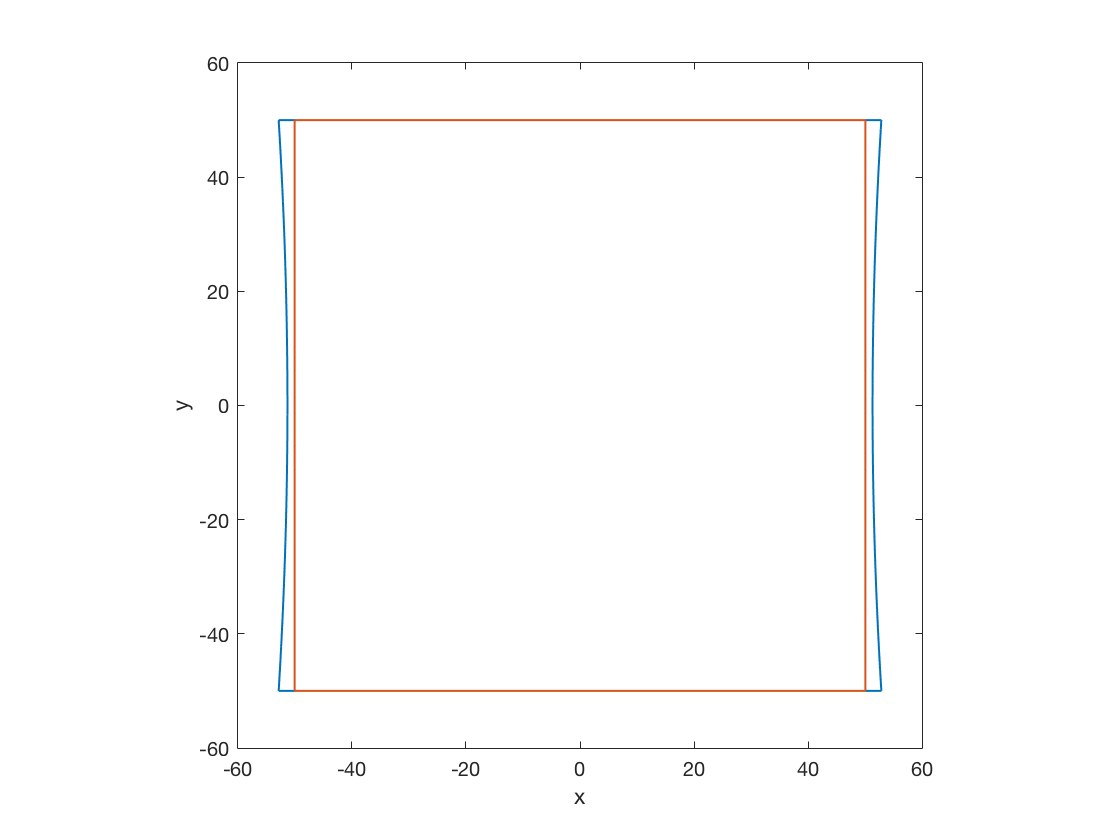
\includegraphics[width=\linewidth]{MG7.png}
\caption{Matlab仿真结果,橙色为预期图形,蓝色为实际扫描图形}
\end{figure}
\subsubsection{振镜控制实现}
解释从串口接收的G代码 若需要移动XY振镜及开关激光 则根据依据设置的每秒插补次数对运动的路径进行分割,对每个插补的XY轴分别计算角度,后转换成DA数值,储存在两个数组中,最后使用定时器让振镜在某个细分时间点运动到DA值制定的位置,这样便完成了直线的扫描.由于计算量比较大,使用了一种机制:在运动时(定时器空隙)接收并计算下一个指令,使两个指令间隔时间减少.
本项目使用的一款振镜电机接收模拟信号为0-5V对应-20°至20°,Arduino Due通过SPI与DAC8852(双路)以50M的速度进行通信,将DA值(DAC8552为16位0-5V对应0-65536)发送给DAC模块.
\subsection{步进电机控制理论及实现}
对于SLS3D打印机来说,一共需要控制3个轴:A轴(铺份刮刀),B轴(粉末储存缸),C轴(打印缸)来完成铺粉过程\\
通过脉冲控制步进电机,脉冲间隔决定电机旋转速度,需要考虑电机的加减速,否则电机将很容易失步
\begin{figure}[ht]
\centering     
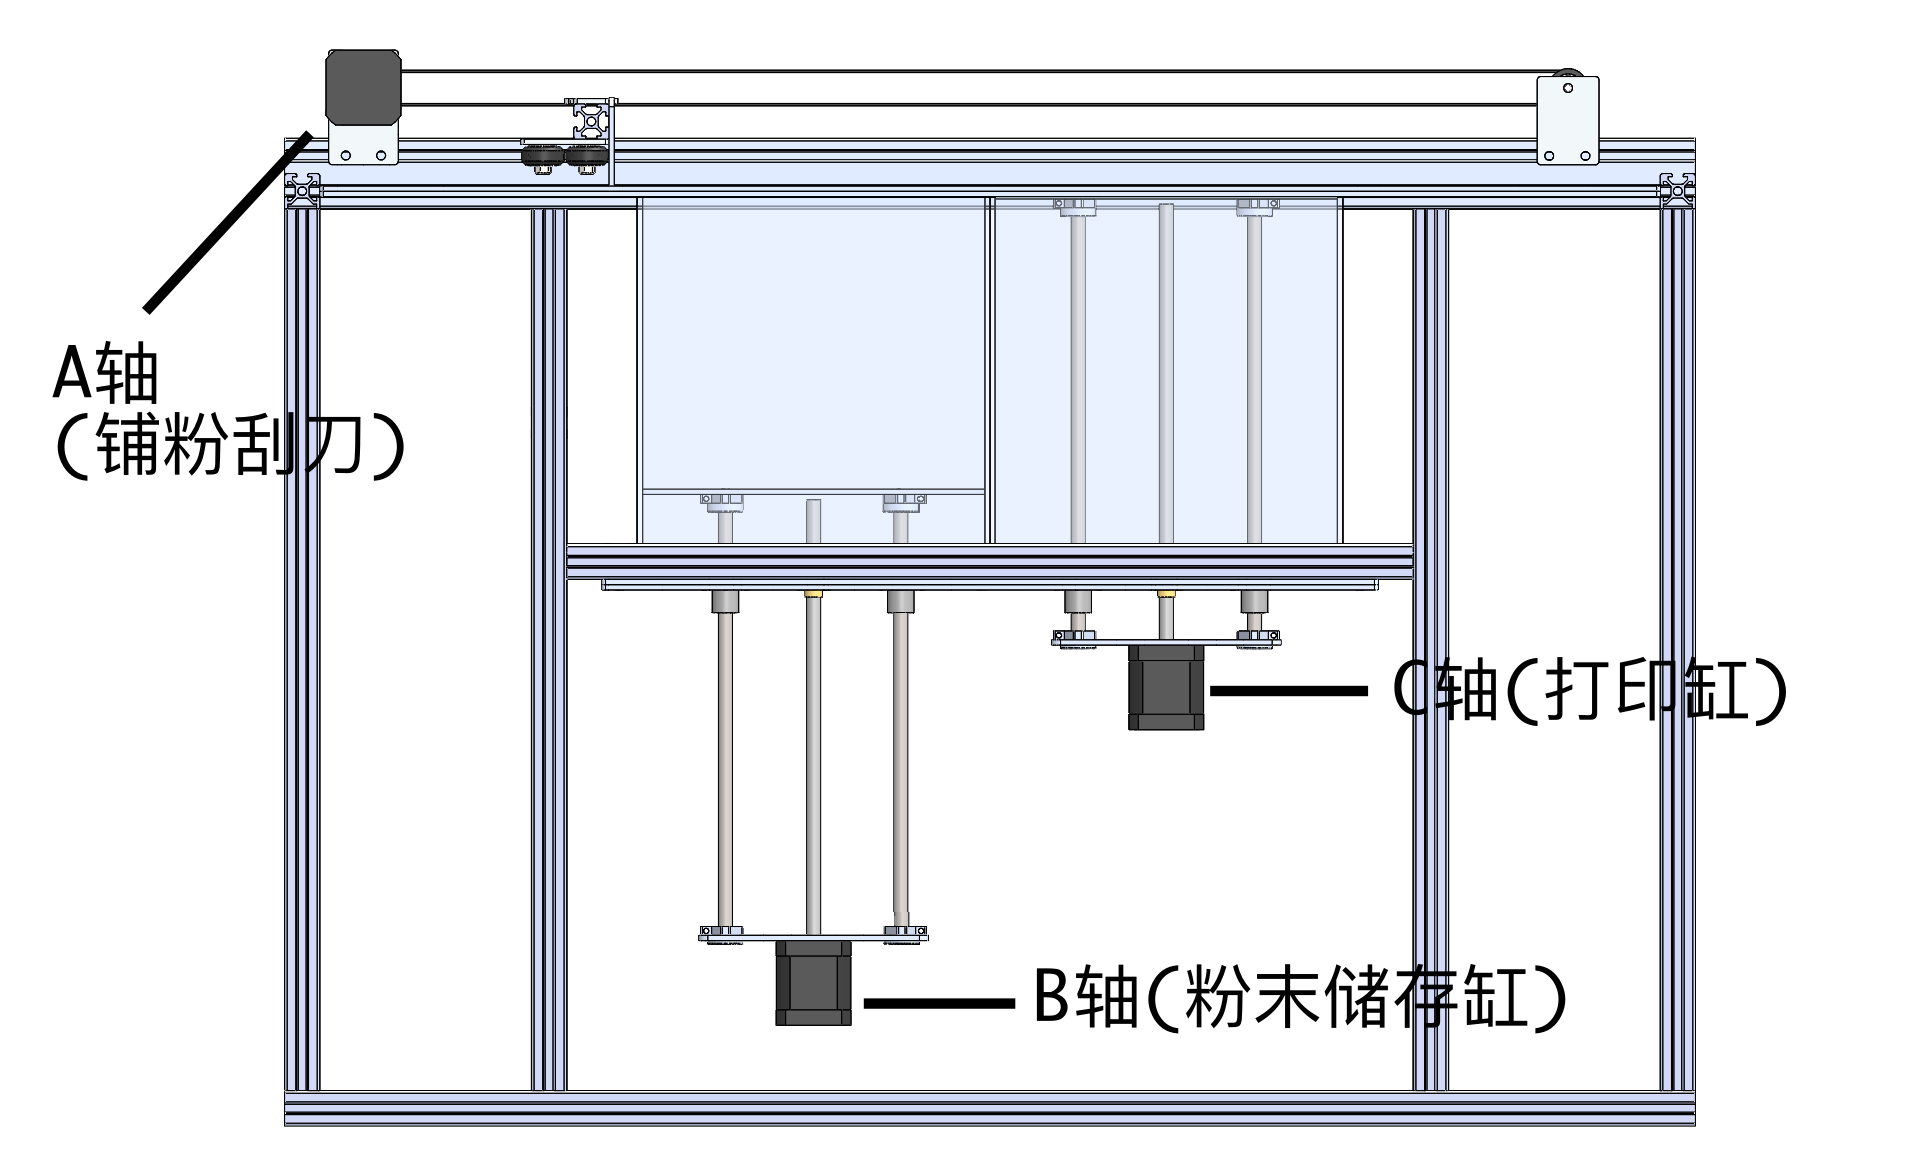
\includegraphics[width=\linewidth]{stepper.png}
\caption{三个直线运动轴}
\end{figure}
\subsubsection{单轴步进电机加减速控制}
\paragraph{条件}
$S$为加速距离(单位:$step$),
$a$为加速度(单位:$step/s^2$),
$v_0$为初始速度(单位:$step/s$),
$v$为目标速度(单位:$step/s$),	
$t$为加速度时间(单位:$s$)
\subparagraph{运动学}{
}
\begin{equation}
s=\frac{v^2-v_0^2}{2a}
\end{equation}
\begin{equation}
v=\sqrt{v_0^2+2aS}
\end{equation}
设$i$为第几步
\begin{equation}
v_i=\sqrt{v_{i-1}^2+2a}
\end{equation}
\paragraph{控制}
使用定时器控制脉冲发送间隔 设:
$P_i$为第i步的间隔时间(单位:$ticks$)
$F$为定时器唤醒周期(单位$ticks/s$)
\begin{equation}
P_i=F/v_i 
\end{equation}
由$(13)$和$(14)$得:
\begin{equation}
P_i=\frac{F}{\sqrt{\frac{F}{P_{i-1}}}^2+2a}
\end{equation}
即
\begin{equation}
P_i=\frac{P_{i-1}}{\sqrt{1+\frac{P_{i-1}^2 2 a}{F^2}}}
\end{equation}

\subparagraph{化简}泰勒展开在$-1\leq n \leq 1$时
\\$\frac{1}{\sqrt{1+n}}\approx1-\frac{n}{2}$
 所以
\begin{equation}
 P_i=P_{i-1}(1-\frac{P_{i-1}^2a}{F^2})
\end{equation}
而$a$ $F^2$为常数
\subsubsection{步进电机控制实现}
在$(17)$中,而$a$ $F^2$在加速度不变时为常量,在程序编译或者控制板开启时可以预先计算在后面的运算中作为常量乘子参与运算\\设$R=\frac{a}{F^2}$则有\\
初始化:
\begin{equation}
P=\frac{F}{\sqrt{V_0^2+2a}}
\end{equation}
加速时:
\begin{equation}
P=P(1-RP^2)
\end{equation}
到达目标速度时:
\begin{equation}
P=P
\end{equation}
减速时:
\begin{equation}
P=P(1+RP^2)
\end{equation}
除了初始化,其他计算只有乘法和加法,因此效率很高.\\
在控制板开启时初始化,计算出第一次的脉冲时间间隔,设定定时器,每次被定时器唤醒就发送一个脉冲并计算下一个脉冲间隔时间,并根据计算出来的脉冲设定定时器的唤醒间隔.
\newpage
\section{机械设计}
本章介绍SLS3D打印机的机械结构都使用Solidworks建模装配\\
一共开发了三代原型机,一个实验平台,将着重介绍第三代.细节详见公开的solidworks源文件
\begin{figure}[ht]
\centering     
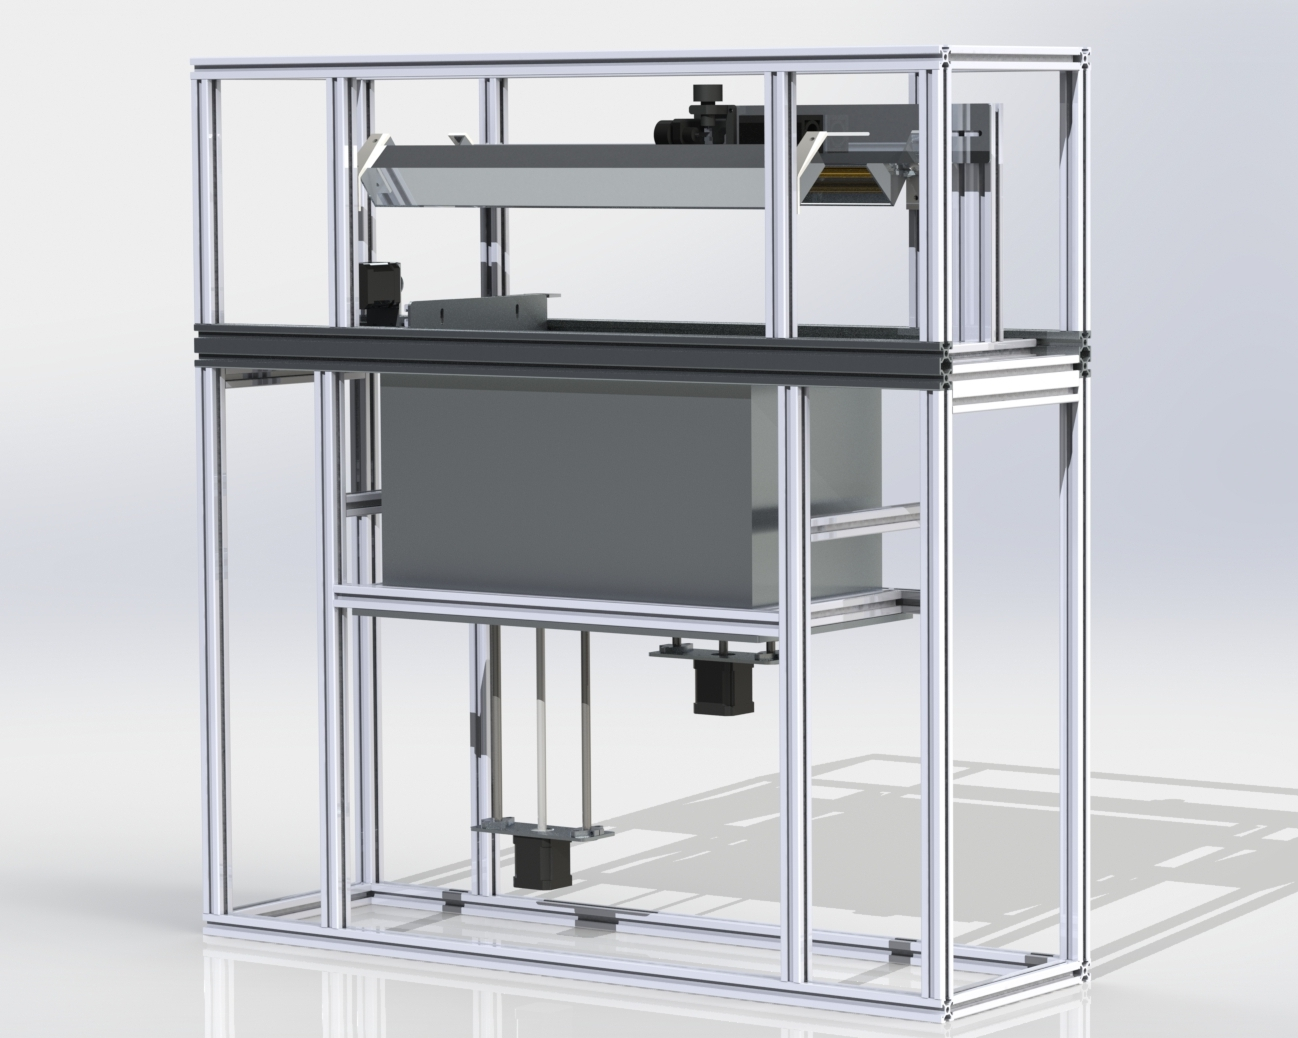
\includegraphics[width=\linewidth]{MGSLS3_0.jpg}
\caption{第三代打印机渲染图}
\end{figure}
\subsection{前代打印机}
\paragraph{第一代}
40WCO2激光管 激光振镜 亚克力及铝型材搭建的Z轴
此版本的因为设计时没有考虑到CO2激光功率过大,需要水冷,亚克力不耐热等问题无法使用.\\
\begin{figure}[ht]
\centering     
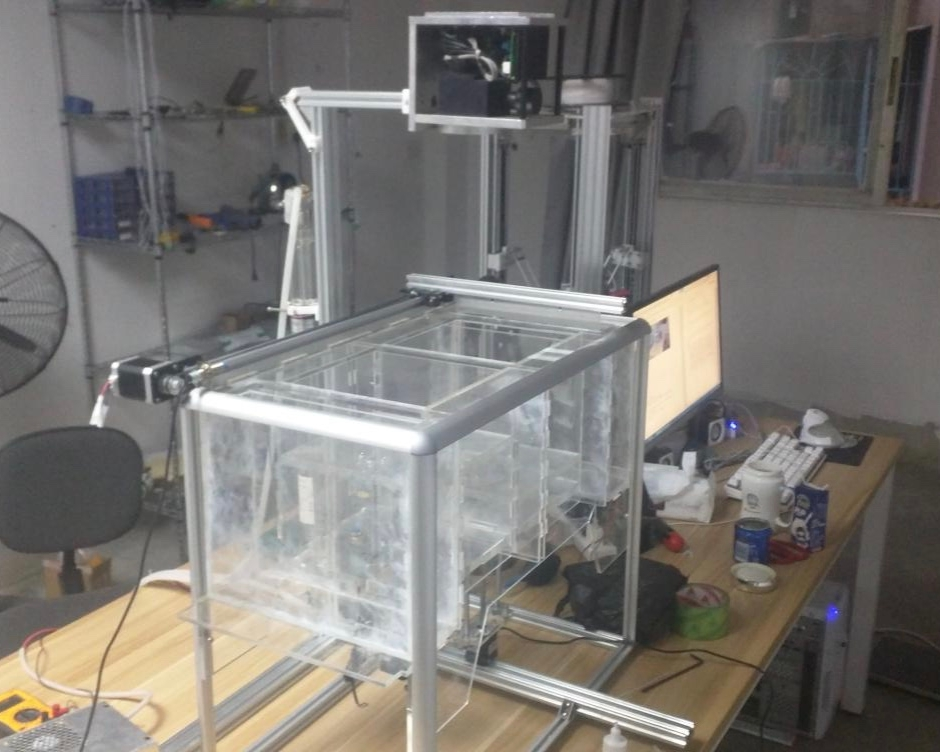
\includegraphics[width=0.8\linewidth]{MGSLS1_0.jpg}
\caption{第一代打印机实物图}
\end{figure}
\newpage
\paragraph{第二代}
使用半导体激光 激光振镜 铝板 铝型材搭建的第二代原型机
\begin{figure}[ht]
\centering     
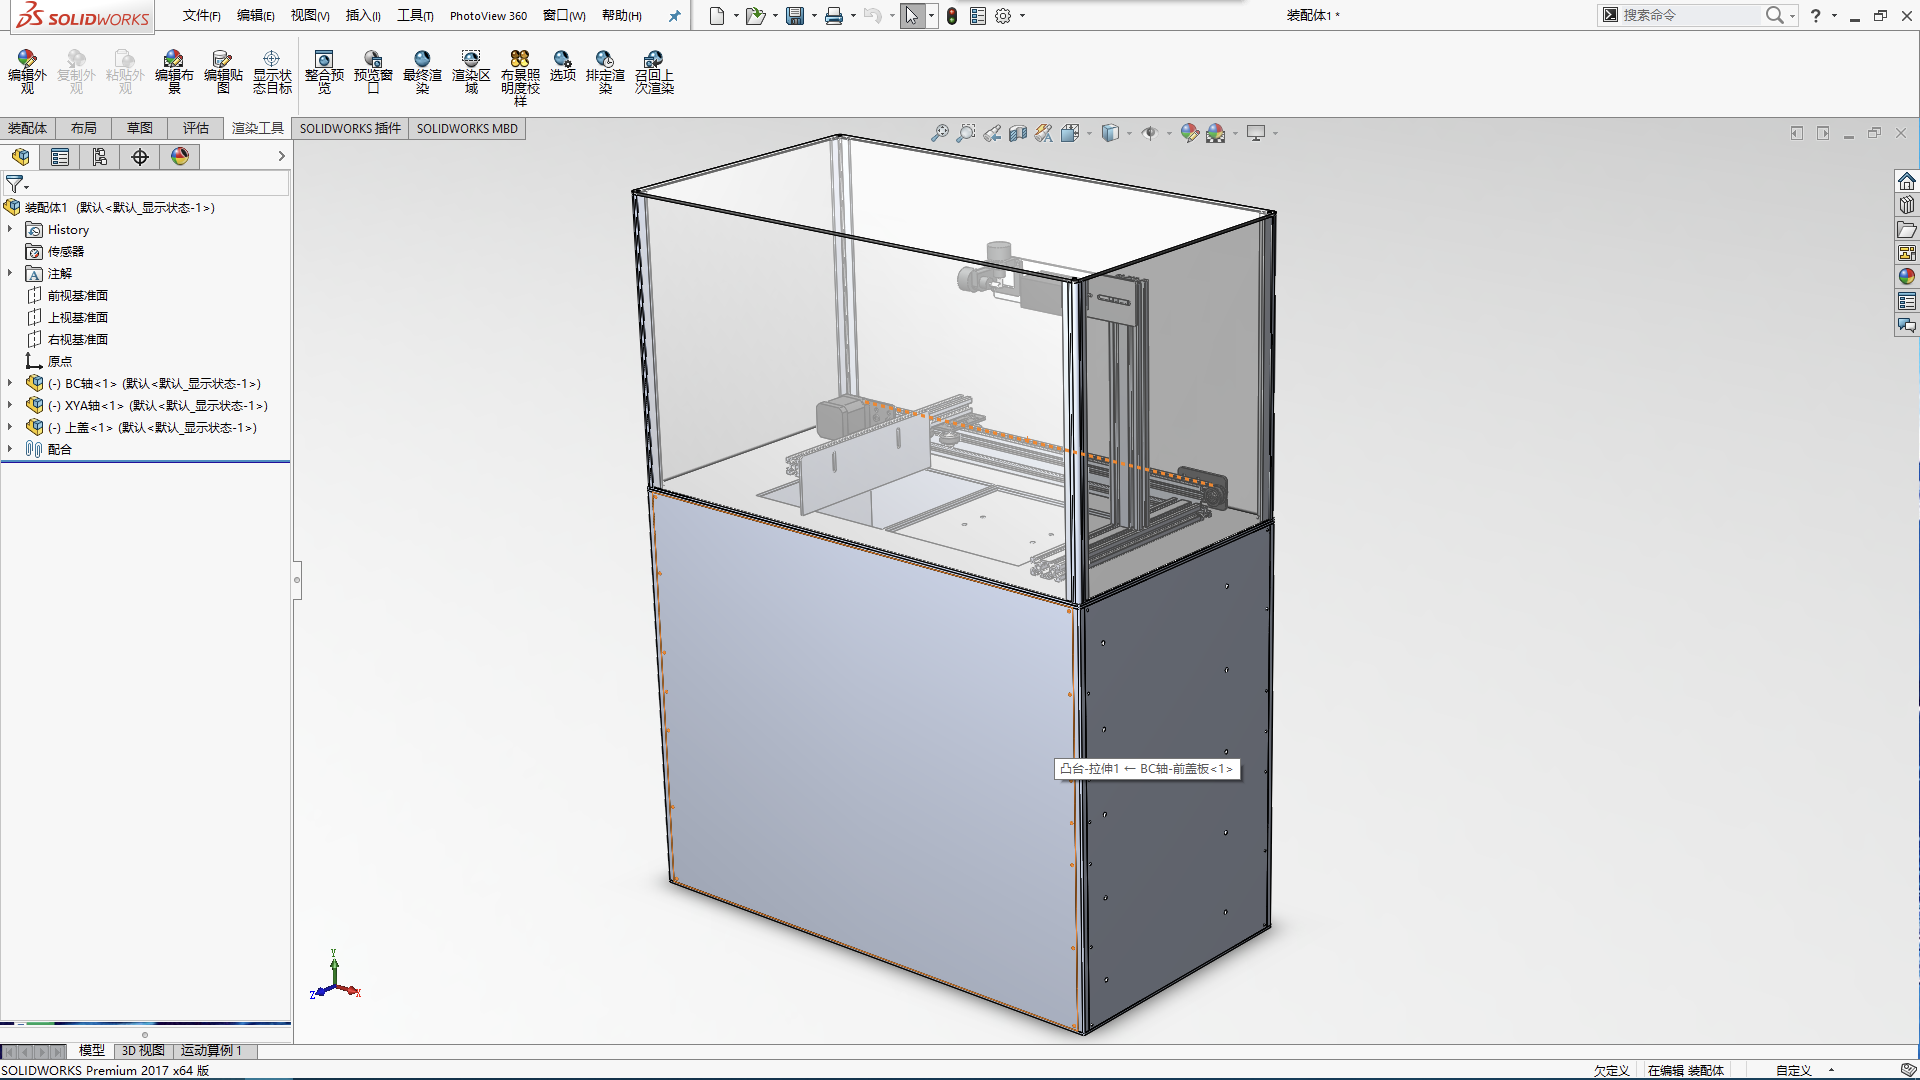
\includegraphics[width=0.8\linewidth]{MGSLS2_0.png}
\centering     
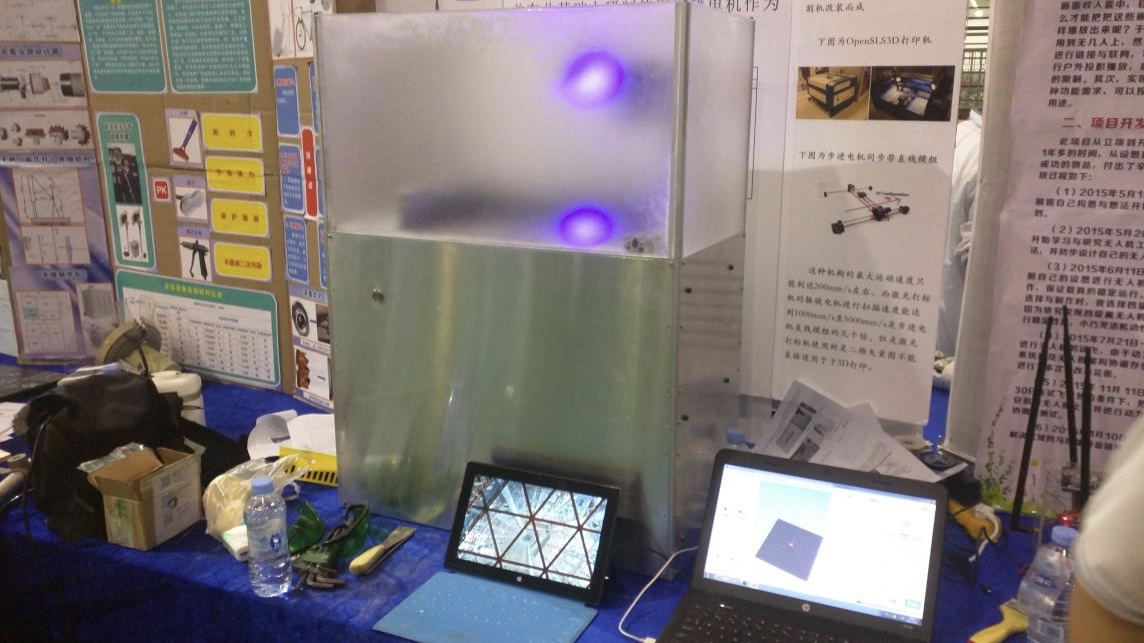
\includegraphics[width=0.8\linewidth]{MGSLS2_1.jpg}
\caption{第二代打印机渲染图及实物图}
\end{figure}
\subsection{二维烧结实验平台}
二维烧结实验平台用于单层烧结实验,使用5W半导体激光(450nm)及激光振镜,并在底部加装加热板对粉末预热
\begin{figure}[ht]
\centering     
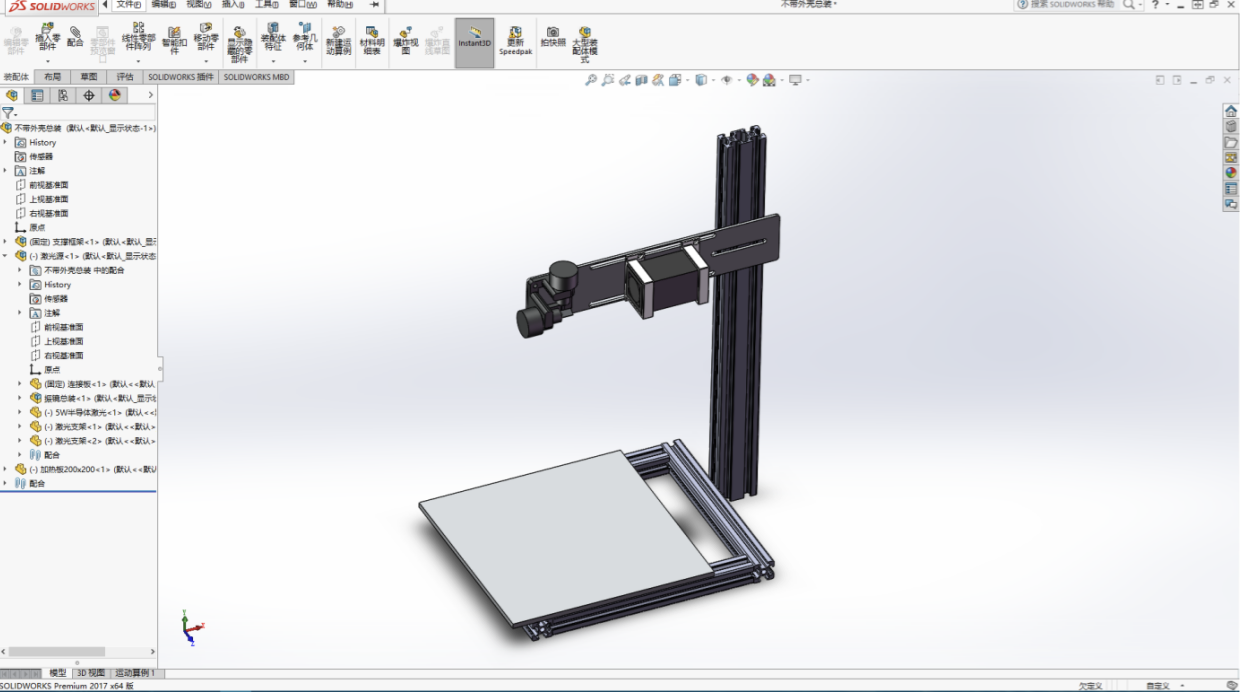
\includegraphics[width=0.8\linewidth]{MGSLS0_0.png}
\centering     
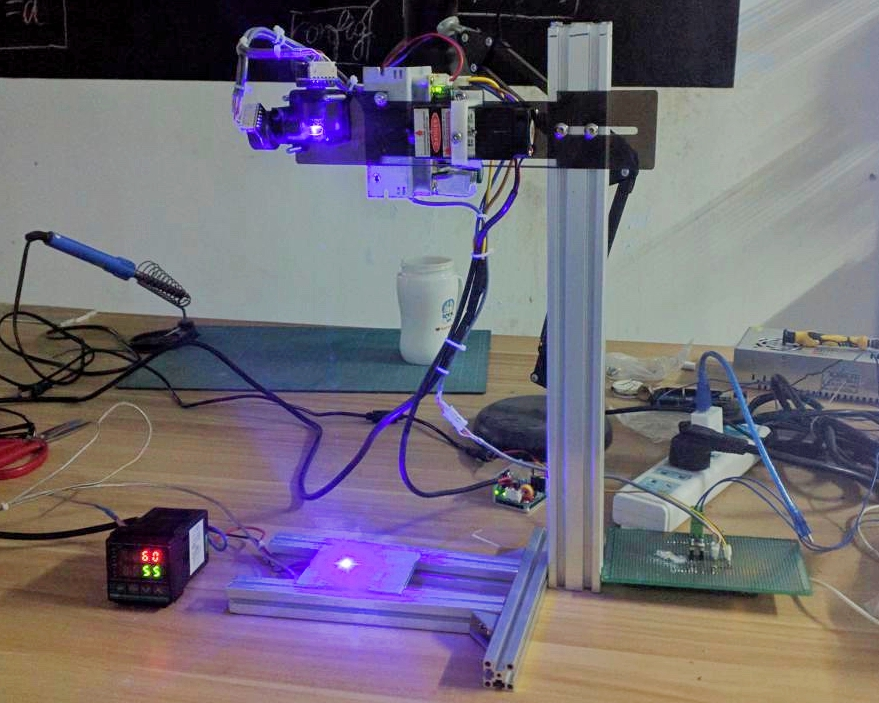
\includegraphics[width=0.8\linewidth]{MGSLS0_1.jpg}
\caption{二维烧结实验平台模型图及实物图}
\end{figure}
\newpage
\subsection{第三代SLS打印机}
打印机由三部分构成:\\
激光机构(XY轴)\\
粉末机构(ABC轴)\\
加热机构
\paragraph{激光机构}
激光机构由两个振镜电机依照上章所述的方式安装,使用了一个5W450nm半导体激光器.
\begin{figure}[ht]
\centering
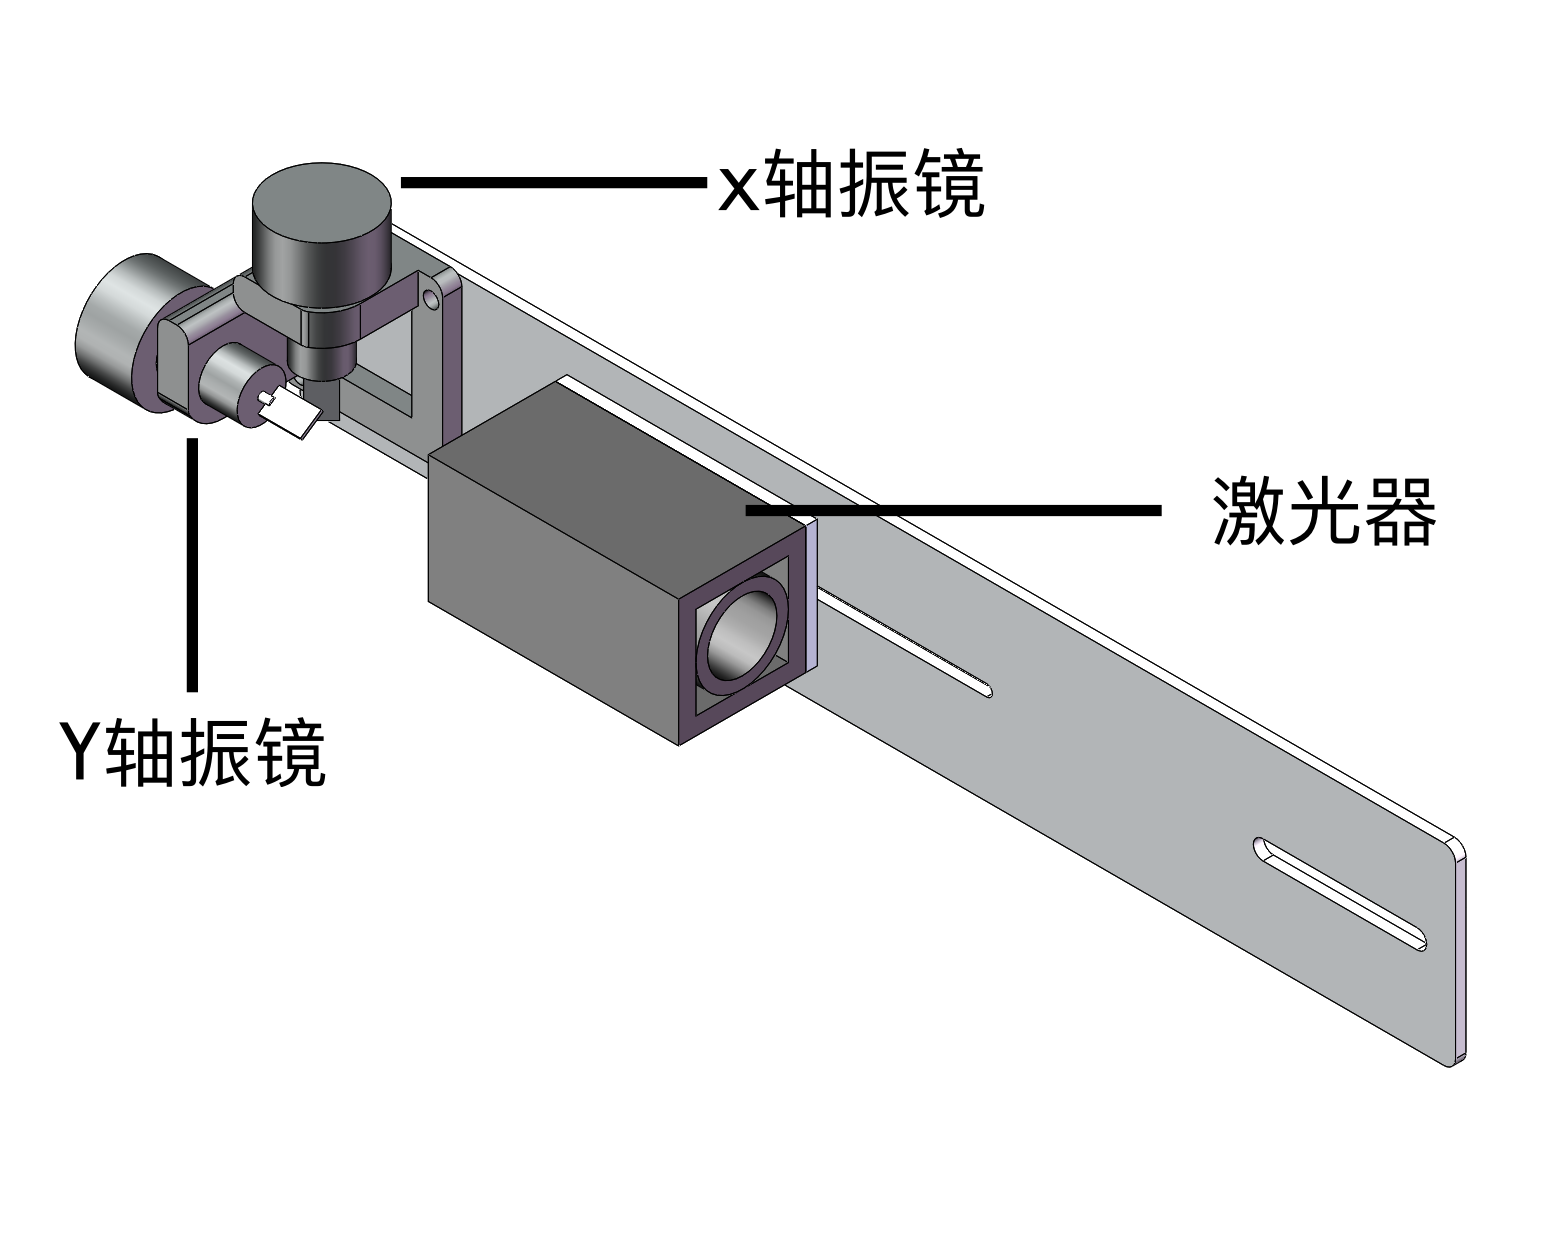
\includegraphics[width=\linewidth]{MGSLS3_2.png}
\caption{激光机构}
\end{figure}
\paragraph{粉末机构}
粉末机构的作用是覆盖一层粉末到已烧结完成的打印件上面,从而完成整个三维堆积的过程\\
具体的过程如下:\\初始状态时,粉末储存缸(B轴)的推杆降到最低,而打印缸推杆(C轴)上升到距离缸口极小的距离,将两个缸都装满粉,刮刀往返运动一次,这时打印缸内便有了一层薄而又均匀的粉末,进行平面烧结后,打印缸下降一段距离,粉末储存缸上升一段距离,这时便有部分粉末从粉末储存缸的缸口溢出,刮刀往返一次,将粉末储存缸的粉末带到打印缸,并铺匀,这时,第一次平面烧结得到的打印件上面便覆盖了一层粉末,继续扫描,扑粉,不断重复这个过程.
\begin{figure}[ht]
\centering
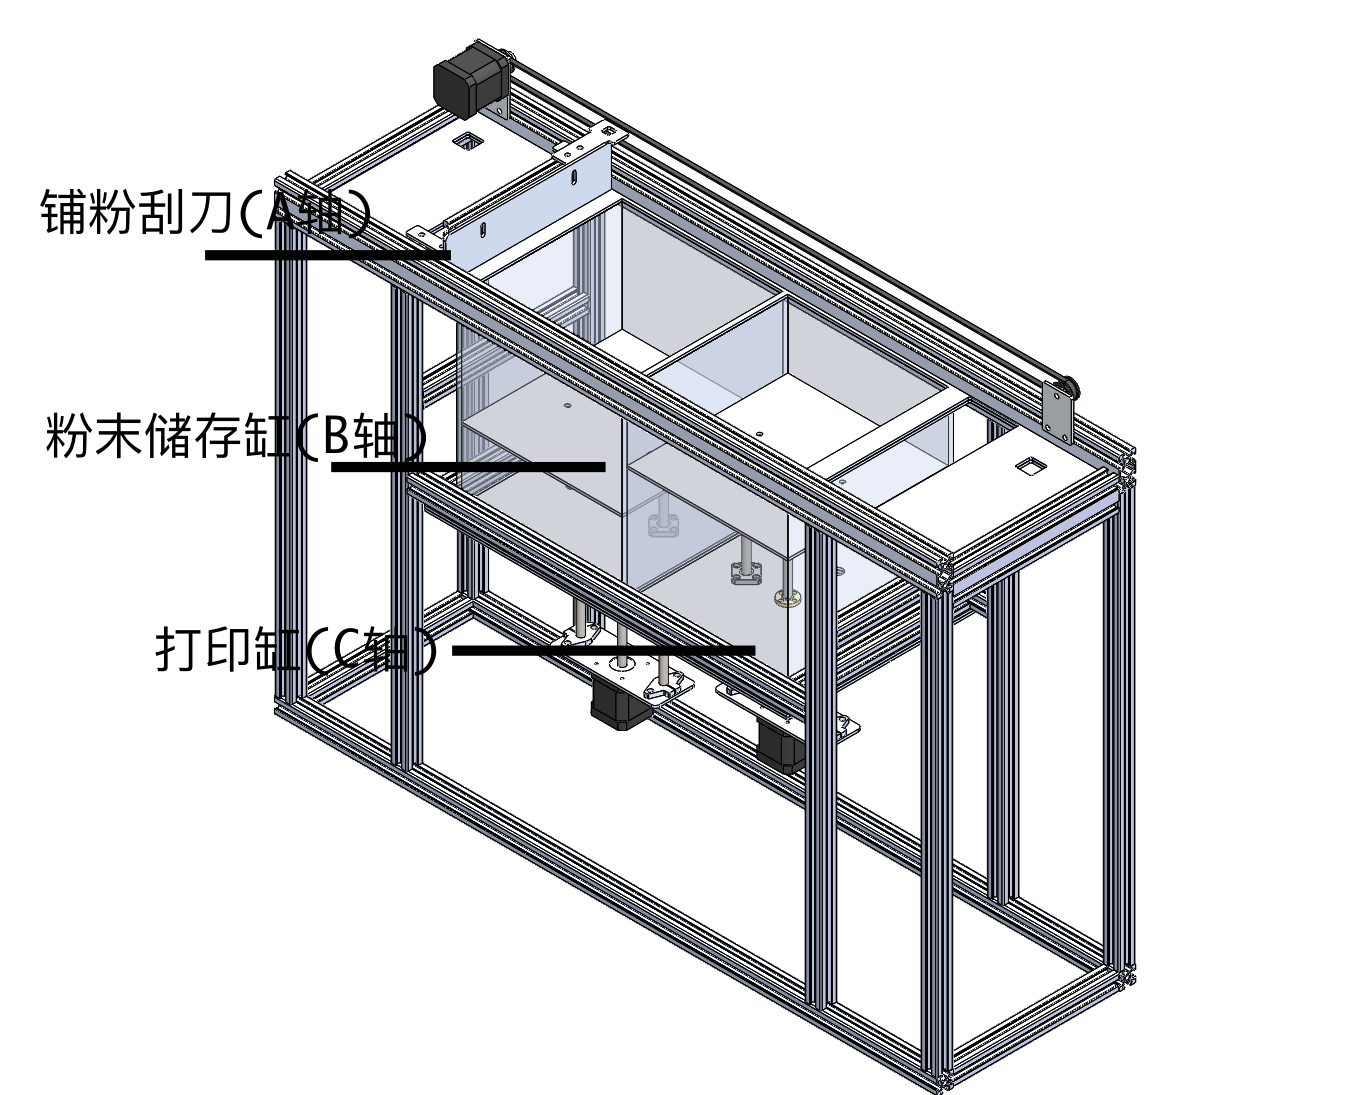
\includegraphics[width=0.75\linewidth]{MGSLS3_1.png}
\caption{ 粉末机构}
\end{figure}
\newpage
\paragraph{加热机构}
使用两个红外加热管对粉末进行预热
\begin{figure}[ht]
\centering
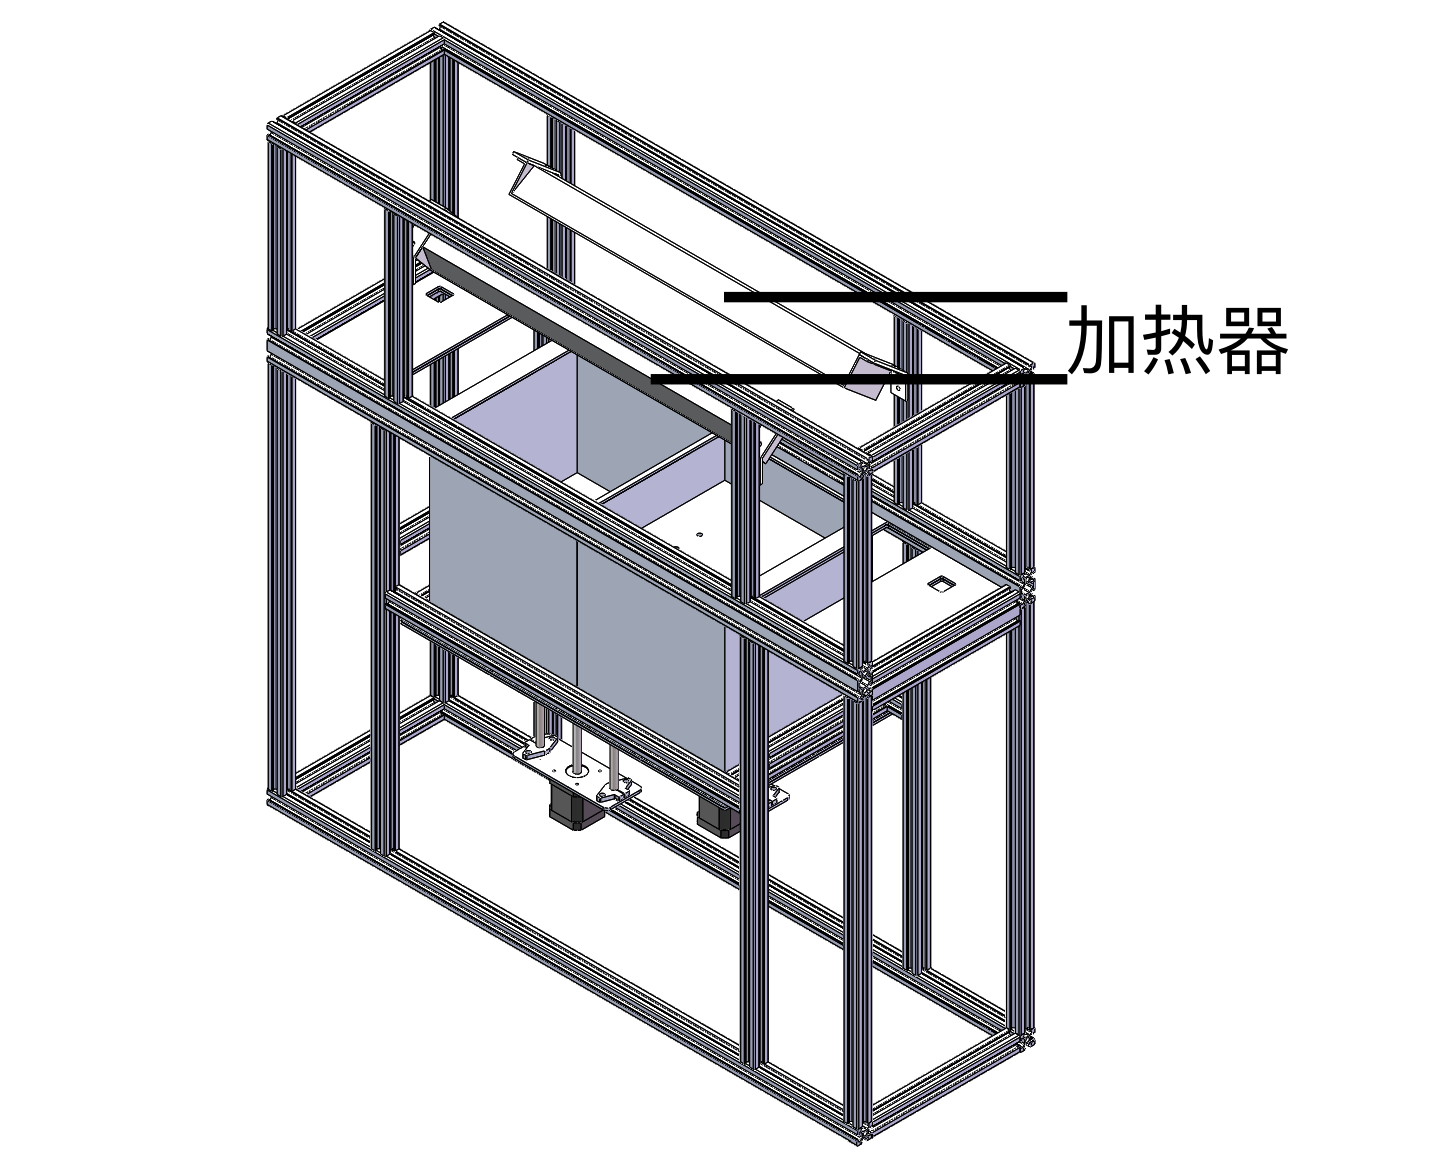
\includegraphics[width=0.8\linewidth]{MGSLS3_3.png}
\caption{加热机构}
\end{figure}
\paragraph{整机}整机模型图
\begin{figure}[ht]
\centering
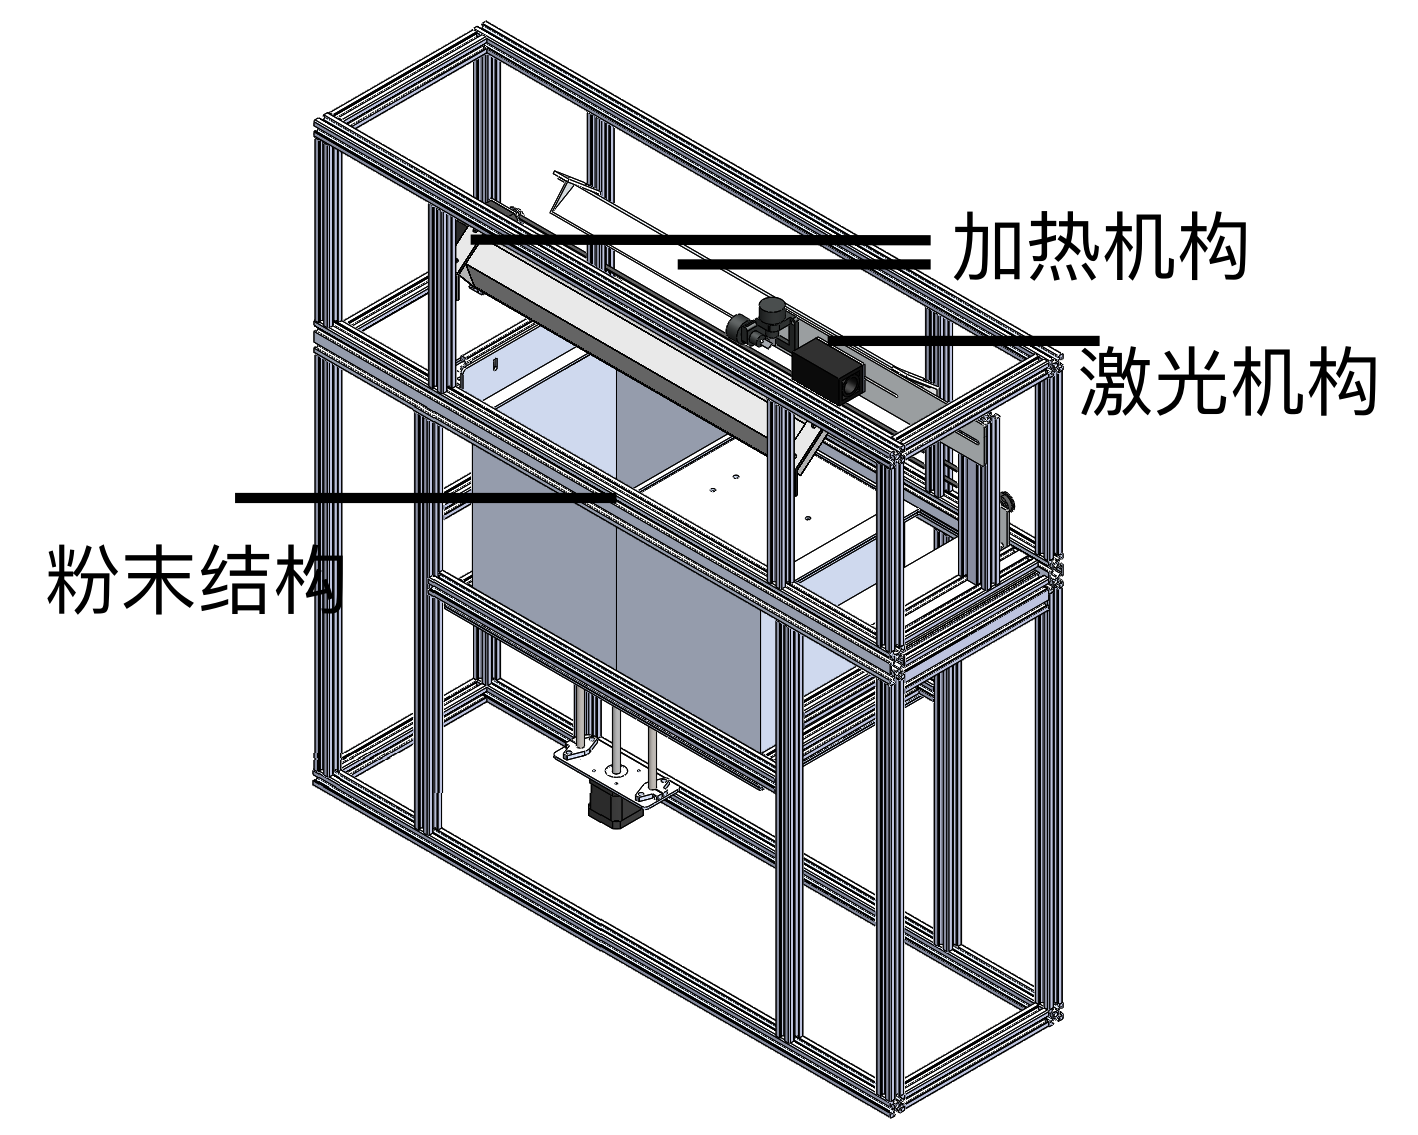
\includegraphics[width=0.8\linewidth]{MGSLS3_4.png}
\caption{整机}
\end{figure}

%结构
\newpage
\section{结果}
\paragraph{单层烧结}
\subparagraph{扫描性能}
在不考虑激光功率的情况下,振镜电机在GCode的控制下速度可以达到1000mm/s至5000mm/s,速度越快,精度越低.
\subparagraph{烧结结果}
使用XY测试平台使用黑色碳粉末和白色PLA粉末混合,增加激光被吸收的热量,进行单层烧结实验,可以得到精密结合的薄塑料片.
\begin{figure}[ht]
\centering
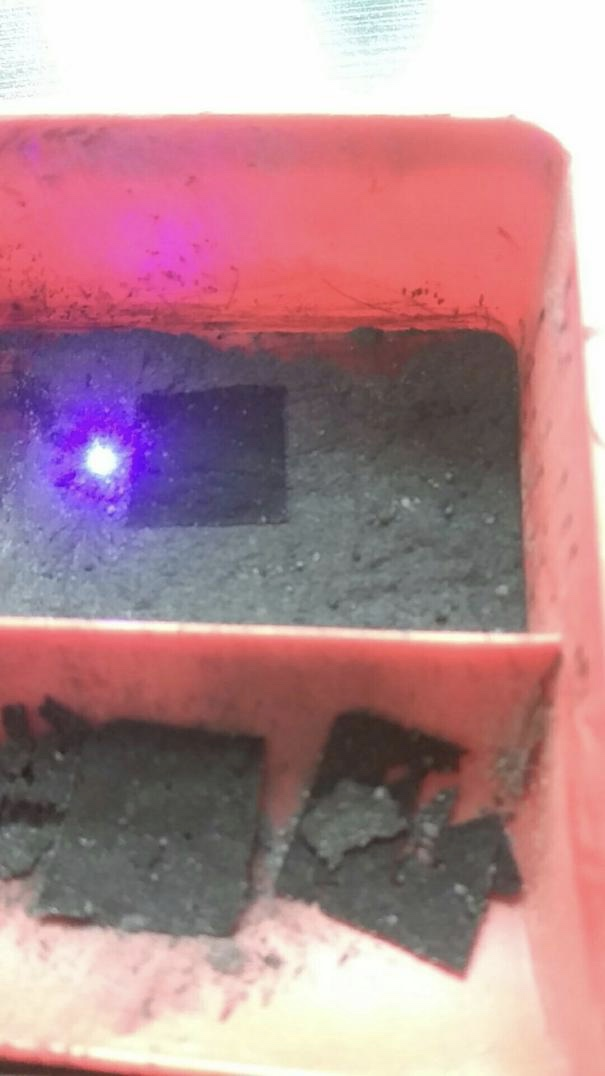
\includegraphics[width=0.45\linewidth]{result0.jpg}
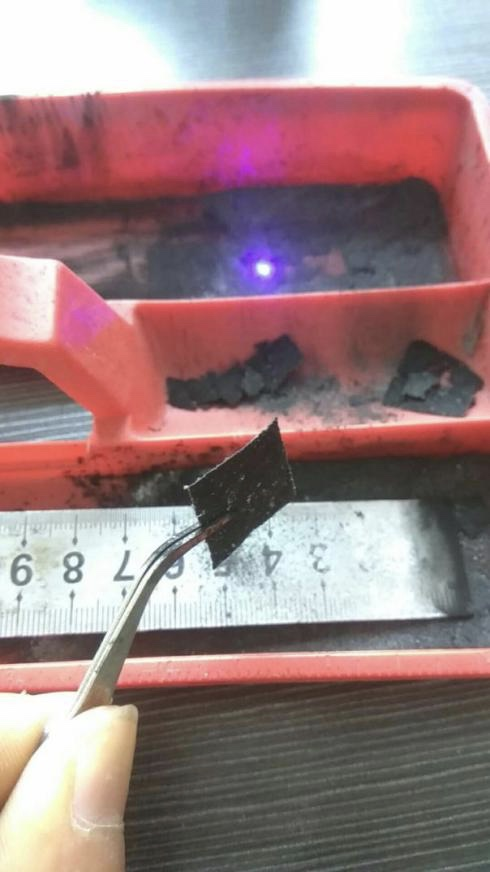
\includegraphics[width=0.45\linewidth]{result1.jpg}
\caption{单层烧结}
\end{figure}

\paragraph{多层烧结(即3D打印)}
使用第三代打印机对粉末进行进行多层烧结,层与层之间粘黏良好,可以打印出许多结构及其复杂(其他打印机无法打印出来)的模型.
\begin{figure}[ht]
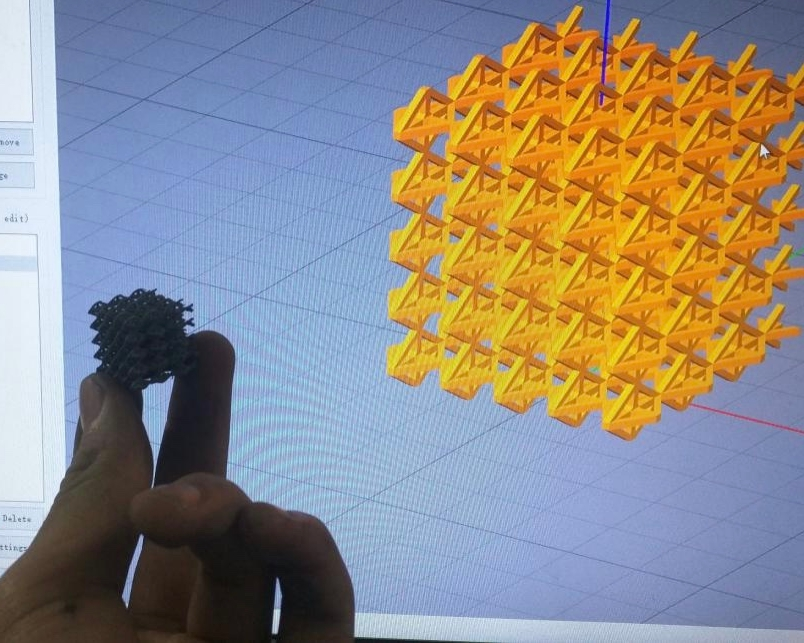
\includegraphics[width=0.49\linewidth]{result2.jpg}
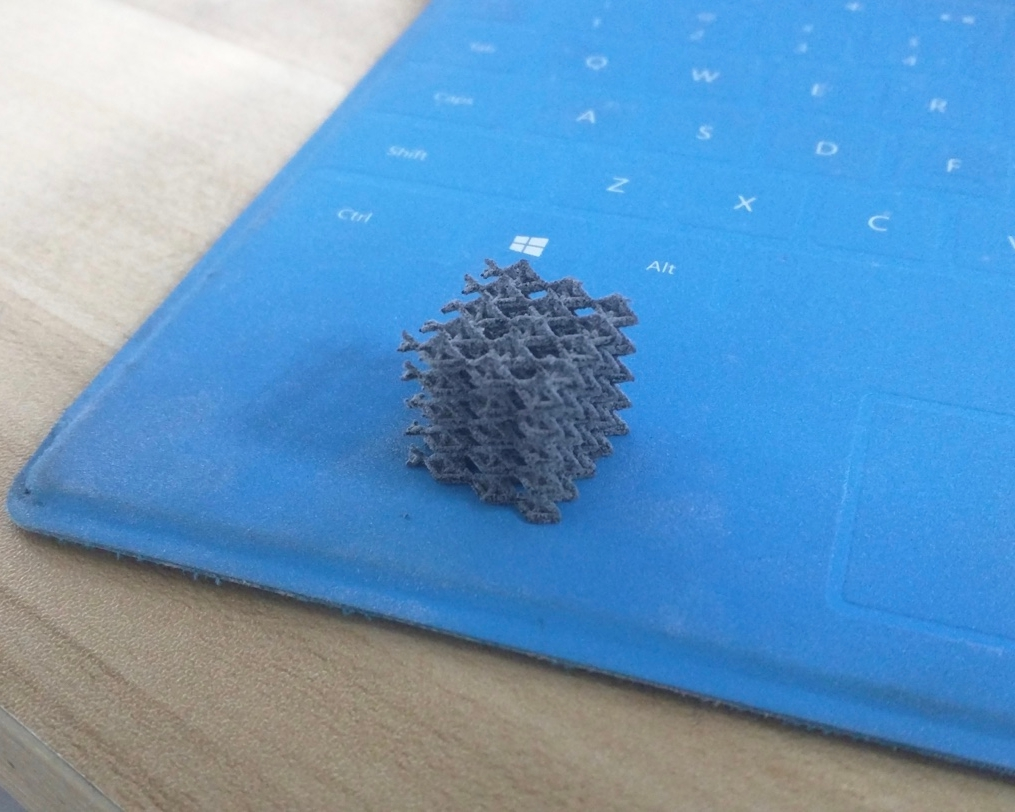
\includegraphics[width=0.49\linewidth]{result3.jpg}
\caption{多层烧结(3D打印)}
\end{figure}
\newpage
%结论
\section{结论}
本项目成功开发一个运行在Arduino Due单片机上的控制系统,可以用数控设备通用的G代码控制振镜,使得振镜电机组兼容常规3D切片软件,可以用于SLS3D打印,并在此基础上开发使用振镜电机作为XY轴的桌面级SLS3D打印机,并使用腌制出来的SLS3D打印机成功打印出塑料打印件\\
作为一个系统,在根据不同材料要求更换激光器的功率波长后,理论上可以兼容其他材料,如金属,铸造蜡,光敏树脂等.
%致谢
\section{致谢}

%参考文献
\section{参考文献}
赵毅, 卢秉恒. 振镜扫描系统的枕形畸变校正算法[J]. 中国激光, 2003, 30(3): 216-218.\\
Eiderman A. Real Time Stepper Motor Linear Ramping Just by Addition and Multiplication[J].\\
\end{document}
